\documentclass{book}
\usepackage[a4paper,top=2.5cm,bottom=2.5cm,left=2.5cm,right=2.5cm]{geometry}
\usepackage{makeidx}
\usepackage{natbib}
\usepackage{graphicx}
\usepackage{multicol}
\usepackage{float}
\usepackage{listings}
\usepackage{color}
\usepackage{ifthen}
\usepackage[table]{xcolor}
\usepackage{textcomp}
\usepackage{alltt}
\usepackage{ifpdf}
\ifpdf
\usepackage[pdftex,
            pagebackref=true,
            colorlinks=true,
            linkcolor=blue,
            unicode
           ]{hyperref}
\else
\usepackage[ps2pdf,
            pagebackref=true,
            colorlinks=true,
            linkcolor=blue,
            unicode
           ]{hyperref}
\usepackage{pspicture}
\fi
\usepackage[utf8]{inputenc}
\usepackage{mathptmx}
\usepackage[scaled=.90]{helvet}
\usepackage{courier}
\usepackage{sectsty}
\usepackage{amssymb}
\usepackage[titles]{tocloft}
\usepackage{doxygen}
\lstset{language=C++,inputencoding=utf8,basicstyle=\footnotesize,breaklines=true,breakatwhitespace=true,tabsize=4,numbers=left }
\makeindex
\setcounter{tocdepth}{3}
\renewcommand{\footrulewidth}{0.4pt}
\renewcommand{\familydefault}{\sfdefault}
\hfuzz=15pt
\setlength{\emergencystretch}{15pt}
\hbadness=750
\tolerance=750
\begin{document}
\hypersetup{pageanchor=false,citecolor=blue}
\begin{titlepage}
\vspace*{7cm}
\begin{center}
{\Large C\-L Tp1 \\[1ex]\large 1.\-0 }\\
\vspace*{1cm}
{\large Generated by Doxygen 1.8.2}\\
\vspace*{0.5cm}
{\small Mon Nov 25 2013 12:48:13}\\
\end{center}
\end{titlepage}
\clearemptydoublepage
\pagenumbering{roman}
\tableofcontents
\clearemptydoublepage
\pagenumbering{arabic}
\hypersetup{pageanchor=true,citecolor=blue}
\chapter{Main Page}
\label{index}\hypertarget{index}{}\subsection*{Conception de Langage}

T\-E\-X\-T\-E

\subsection*{Sash Project}

This project consists in adding two evaluators in Sash project. 
\chapter{Hierarchical Index}
\section{Class Hierarchy}
This inheritance list is sorted roughly, but not completely, alphabetically\-:\begin{DoxyCompactList}
\item \contentsline{section}{Abstract\-Number}{\pageref{class_abstract_number}}{}
\begin{DoxyCompactList}
\item \contentsline{section}{Number}{\pageref{class_number}}{}
\end{DoxyCompactList}
\item \contentsline{section}{Boolean\-Condition}{\pageref{class_boolean_condition}}{}
\begin{DoxyCompactList}
\item \contentsline{section}{Binary\-Boolean\-Condition}{\pageref{class_binary_boolean_condition}}{}
\begin{DoxyCompactList}
\item \contentsline{section}{A\-N\-D}{\pageref{class_a_n_d}}{}
\item \contentsline{section}{O\-R}{\pageref{class_o_r}}{}
\end{DoxyCompactList}
\item \contentsline{section}{Binary\-Number\-Condition}{\pageref{class_binary_number_condition}}{}
\begin{DoxyCompactList}
\item \contentsline{section}{Less\-Than\-Or\-Equal}{\pageref{class_less_than_or_equal}}{}
\end{DoxyCompactList}
\item \contentsline{section}{Unary\-Boolean\-Condition}{\pageref{class_unary_boolean_condition}}{}
\begin{DoxyCompactList}
\item \contentsline{section}{Boolean}{\pageref{class_boolean}}{}
\item \contentsline{section}{N\-O\-T}{\pageref{class_n_o_t}}{}
\end{DoxyCompactList}
\end{DoxyCompactList}
\item \contentsline{section}{Context}{\pageref{class_context}}{}
\begin{DoxyCompactList}
\item \contentsline{section}{Global\-Context}{\pageref{class_global_context}}{}
\end{DoxyCompactList}
\item \contentsline{section}{Expression}{\pageref{class_expression}}{}
\begin{DoxyCompactList}
\item \contentsline{section}{Function}{\pageref{class_function}}{}
\item \contentsline{section}{If\-Then\-Else}{\pageref{class_if_then_else}}{}
\item \contentsline{section}{Number}{\pageref{class_number}}{}
\item \contentsline{section}{Operation}{\pageref{class_operation}}{}
\begin{DoxyCompactList}
\item \contentsline{section}{Add}{\pageref{class_add}}{}
\item \contentsline{section}{Divide}{\pageref{class_divide}}{}
\item \contentsline{section}{Modulo}{\pageref{class_modulo}}{}
\item \contentsline{section}{Substract}{\pageref{class_substract}}{}
\item \contentsline{section}{Time}{\pageref{class_time}}{}
\end{DoxyCompactList}
\item \contentsline{section}{Variable}{\pageref{class_variable}}{}
\end{DoxyCompactList}
\item \contentsline{section}{Factory}{\pageref{class_factory}}{}
\item \contentsline{section}{Global\-Functions}{\pageref{class_global_functions}}{}
\end{DoxyCompactList}

\chapter{Class Index}
\section{Class List}
Here are the classes, structs, unions and interfaces with brief descriptions\-:\begin{DoxyCompactList}
\item\contentsline{section}{\hyperlink{class_abstract_number}{Abstract\-Number} \\*Abstraction of a \hyperlink{class_number}{Number} }{\pageref{class_abstract_number}}{}
\item\contentsline{section}{\hyperlink{class_add}{Add} \\*\hyperlink{class_add}{Add} operation }{\pageref{class_add}}{}
\item\contentsline{section}{\hyperlink{class_a_n_d}{A\-N\-D} \\*And combination }{\pageref{class_a_n_d}}{}
\item\contentsline{section}{\hyperlink{class_binary_boolean_condition}{Binary\-Boolean\-Condition} \\*Represents a binary boolean condition. It contains two members }{\pageref{class_binary_boolean_condition}}{}
\item\contentsline{section}{\hyperlink{class_binary_number_condition}{Binary\-Number\-Condition} \\*Represents a boolean condition in whiwh each member is numeral }{\pageref{class_binary_number_condition}}{}
\item\contentsline{section}{\hyperlink{class_boolean}{Boolean} \\*Represents a boolean object (Necesssary for construction of A\-S\-T) }{\pageref{class_boolean}}{}
\item\contentsline{section}{\hyperlink{class_boolean_condition}{Boolean\-Condition} \\*Abstract boolean condition. It should be an expression but is is not to simplify calculus }{\pageref{class_boolean_condition}}{}
\item\contentsline{section}{\hyperlink{class_context}{Context} \\*A context is a mix between the stack and the heap in which variables are stored }{\pageref{class_context}}{}
\item\contentsline{section}{\hyperlink{class_divide}{Divide} \\*\hyperlink{class_divide}{Divide} operation }{\pageref{class_divide}}{}
\item\contentsline{section}{\hyperlink{class_expression}{Expression} \\*Generalized representation of an expression }{\pageref{class_expression}}{}
\item\contentsline{section}{\hyperlink{class_factory}{Factory} \\*\hyperlink{class_factory}{Factory} for creation of all part of the A\-S\-T }{\pageref{class_factory}}{}
\item\contentsline{section}{\hyperlink{class_function}{Function} \\*Represents an A\-S\-T function }{\pageref{class_function}}{}
\item\contentsline{section}{\hyperlink{class_global_context}{Global\-Context} \\*\hyperlink{class_context}{Context} which is always available. This context manages all locals contexts }{\pageref{class_global_context}}{}
\item\contentsline{section}{\hyperlink{class_global_functions}{Global\-Functions} \\*Pool of all evaluated functions }{\pageref{class_global_functions}}{}
\item\contentsline{section}{\hyperlink{class_if_then_else}{If\-Then\-Else} \\*If expression }{\pageref{class_if_then_else}}{}
\item\contentsline{section}{\hyperlink{class_less_than_or_equal}{Less\-Than\-Or\-Equal} \\*A\-S\-T '$<$=' boolean expression }{\pageref{class_less_than_or_equal}}{}
\item\contentsline{section}{\hyperlink{class_modulo}{Modulo} \\*\hyperlink{class_modulo}{Modulo} operation }{\pageref{class_modulo}}{}
\item\contentsline{section}{\hyperlink{class_n_o_t}{N\-O\-T} \\*\hyperlink{class_n_o_t}{N\-O\-T} operator }{\pageref{class_n_o_t}}{}
\item\contentsline{section}{\hyperlink{class_number}{Number} \\*A number is a representation of real world. From outside, there is no difference between integers and floats }{\pageref{class_number}}{}
\item\contentsline{section}{\hyperlink{class_operation}{Operation} \\*A\-S\-T \hyperlink{class_operation}{Operation} }{\pageref{class_operation}}{}
\item\contentsline{section}{\hyperlink{class_o_r}{O\-R} \\*Or combination }{\pageref{class_o_r}}{}
\item\contentsline{section}{\hyperlink{class_substract}{Substract} \\*\hyperlink{class_substract}{Substract} operation }{\pageref{class_substract}}{}
\item\contentsline{section}{\hyperlink{class_time}{Time} \\*\hyperlink{class_time}{Time} operation }{\pageref{class_time}}{}
\item\contentsline{section}{\hyperlink{class_unary_boolean_condition}{Unary\-Boolean\-Condition} \\*Represents an unary boolean condition. It contains one member }{\pageref{class_unary_boolean_condition}}{}
\item\contentsline{section}{\hyperlink{class_variable}{Variable} \\*\hyperlink{class_variable}{Variable} operation }{\pageref{class_variable}}{}
\end{DoxyCompactList}

\chapter{Class Documentation}
\hypertarget{class_abstract_number}{\section{Abstract\-Number Class Reference}
\label{class_abstract_number}\index{Abstract\-Number@{Abstract\-Number}}
}


Abstraction of a \hyperlink{class_number}{Number}.  




Inheritance diagram for Abstract\-Number\-:\nopagebreak
\begin{figure}[H]
\begin{center}
\leavevmode
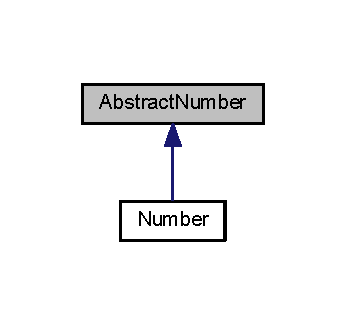
\includegraphics[width=166pt]{class_abstract_number__inherit__graph}
\end{center}
\end{figure}
\subsection*{Public Member Functions}
\begin{DoxyCompactItemize}
\item 
\hypertarget{class_abstract_number_ad228c204b2f3f5bb38d485f0f2181a36}{virtual void {\bfseries set\-Integer} (int val)=0}\label{class_abstract_number_ad228c204b2f3f5bb38d485f0f2181a36}

\item 
\hypertarget{class_abstract_number_a3504505a90056cf3c3386504485efd7a}{virtual void {\bfseries set\-Real} (double val)=0}\label{class_abstract_number_a3504505a90056cf3c3386504485efd7a}

\item 
\hypertarget{class_abstract_number_ac1678d857454b514de3a8ead2578c077}{virtual bool {\bfseries is\-Real} ()=0}\label{class_abstract_number_ac1678d857454b514de3a8ead2578c077}

\item 
\hypertarget{class_abstract_number_a5b68f6e27a691708677d6b8456d79643}{virtual int {\bfseries get\-Integer} ()=0}\label{class_abstract_number_a5b68f6e27a691708677d6b8456d79643}

\item 
\hypertarget{class_abstract_number_aeb63781d71667a7b931637388a91a45f}{virtual double {\bfseries get\-Real} ()=0}\label{class_abstract_number_aeb63781d71667a7b931637388a91a45f}

\item 
\hypertarget{class_abstract_number_a079134fa338f79cbecf7c0c0b0b53327}{virtual std\-::string {\bfseries to\-String} ()=0}\label{class_abstract_number_a079134fa338f79cbecf7c0c0b0b53327}

\item 
\hypertarget{class_abstract_number_a9a3a051700f770168f933cfb5b3220f0}{virtual void {\bfseries from\-String} (std\-::string num)=0}\label{class_abstract_number_a9a3a051700f770168f933cfb5b3220f0}

\item 
\hypertarget{class_abstract_number_ab3fbd477d27fb53fe81e5afabd6639fa}{virtual \hyperlink{class_abstract_number}{Abstract\-Number} $\ast$ {\bfseries eval} ()=0}\label{class_abstract_number_ab3fbd477d27fb53fe81e5afabd6639fa}

\end{DoxyCompactItemize}


\subsection{Detailed Description}
Abstraction of a \hyperlink{class_number}{Number}. 

\begin{DoxyAuthor}{Author}
David Lecoconnier 

Allan Mottier 
\end{DoxyAuthor}
\begin{DoxyDate}{Date}
2013-\/11-\/24 
\end{DoxyDate}


The documentation for this class was generated from the following file\-:\begin{DoxyCompactItemize}
\item 
include/\-Numbers/Abstract\-Number.\-h\end{DoxyCompactItemize}

\hypertarget{class_add}{\section{Add Class Reference}
\label{class_add}\index{Add@{Add}}
}


\hyperlink{class_add}{Add} operation.  




Inheritance diagram for Add\-:\nopagebreak
\begin{figure}[H]
\begin{center}
\leavevmode
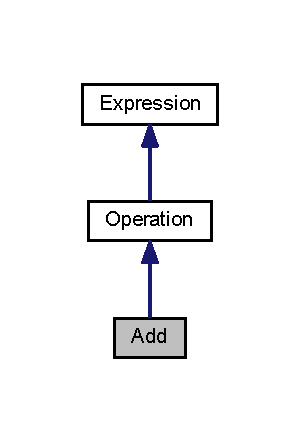
\includegraphics[width=144pt]{class_add__inherit__graph}
\end{center}
\end{figure}


Collaboration diagram for Add\-:\nopagebreak
\begin{figure}[H]
\begin{center}
\leavevmode
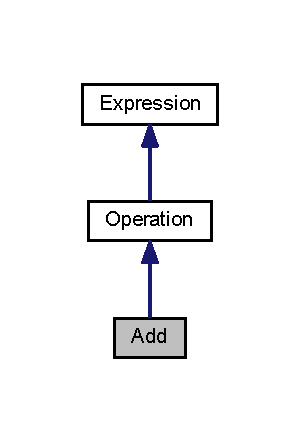
\includegraphics[width=144pt]{class_add__coll__graph}
\end{center}
\end{figure}
\subsection*{Public Member Functions}
\begin{DoxyCompactItemize}
\item 
\hyperlink{class_add_a10e12bf328ba4833ee494f46e4ba879d}{Add} (std\-::string body)
\begin{DoxyCompactList}\small\item\em Default constructor. \end{DoxyCompactList}\item 
virtual \hyperlink{class_add_a960ca471ede083983766bce089f9af64}{$\sim$\-Add} ()
\begin{DoxyCompactList}\small\item\em Default destructor. \end{DoxyCompactList}\item 
virtual \hyperlink{class_abstract_number}{Abstract\-Number} $\ast$ \hyperlink{class_add_a845bcb5bab6962b45a048fd675e3c015}{eval} (std\-::list$<$ \hyperlink{class_expression}{Expression} $\ast$ $>$ $\ast$args)
\begin{DoxyCompactList}\small\item\em Evaluate the \hyperlink{class_add}{Add} operation. \end{DoxyCompactList}\end{DoxyCompactItemize}
\subsection*{Additional Inherited Members}


\subsection{Detailed Description}
\hyperlink{class_add}{Add} operation. 

\begin{DoxyAuthor}{Author}
David Lecoconnier 

Allan Mottier 
\end{DoxyAuthor}
\begin{DoxyDate}{Date}
2013-\/11-\/24 
\end{DoxyDate}


\subsection{Constructor \& Destructor Documentation}
\hypertarget{class_add_a10e12bf328ba4833ee494f46e4ba879d}{\index{Add@{Add}!Add@{Add}}
\index{Add@{Add}!Add@{Add}}
\subsubsection[{Add}]{\setlength{\rightskip}{0pt plus 5cm}Add\-::\-Add (
\begin{DoxyParamCaption}
\item[{std\-::string}]{body}
\end{DoxyParamCaption}
)}}\label{class_add_a10e12bf328ba4833ee494f46e4ba879d}


Default constructor. 

Constructor.


\begin{DoxyParams}{Parameters}
{\em body} & text contained \\
\hline
\end{DoxyParams}
\hypertarget{class_add_a960ca471ede083983766bce089f9af64}{\index{Add@{Add}!$\sim$\-Add@{$\sim$\-Add}}
\index{$\sim$\-Add@{$\sim$\-Add}!Add@{Add}}
\subsubsection[{$\sim$\-Add}]{\setlength{\rightskip}{0pt plus 5cm}Add\-::$\sim$\-Add (
\begin{DoxyParamCaption}
{}
\end{DoxyParamCaption}
)\hspace{0.3cm}{\ttfamily [virtual]}}}\label{class_add_a960ca471ede083983766bce089f9af64}


Default destructor. 

Destructor. 

\subsection{Member Function Documentation}
\hypertarget{class_add_a845bcb5bab6962b45a048fd675e3c015}{\index{Add@{Add}!eval@{eval}}
\index{eval@{eval}!Add@{Add}}
\subsubsection[{eval}]{\setlength{\rightskip}{0pt plus 5cm}{\bf Abstract\-Number} $\ast$ Add\-::eval (
\begin{DoxyParamCaption}
\item[{std\-::list$<$ {\bf Expression} $\ast$ $>$ $\ast$}]{args}
\end{DoxyParamCaption}
)\hspace{0.3cm}{\ttfamily [virtual]}}}\label{class_add_a845bcb5bab6962b45a048fd675e3c015}


Evaluate the \hyperlink{class_add}{Add} operation. 


\begin{DoxyParams}{Parameters}
{\em args} & -\/\-Useless-\/ \\
\hline
\end{DoxyParams}
\begin{DoxyReturn}{Returns}
the result 
\end{DoxyReturn}


Implements \hyperlink{class_expression}{Expression}.



The documentation for this class was generated from the following files\-:\begin{DoxyCompactItemize}
\item 
include/\-Numbers/Add.\-h\item 
src/\-Numbers/Add.\-cpp\end{DoxyCompactItemize}

\hypertarget{class_a_n_d}{\section{A\-N\-D Class Reference}
\label{class_a_n_d}\index{A\-N\-D@{A\-N\-D}}
}


And combination.  




Inheritance diagram for A\-N\-D\-:\nopagebreak
\begin{figure}[H]
\begin{center}
\leavevmode
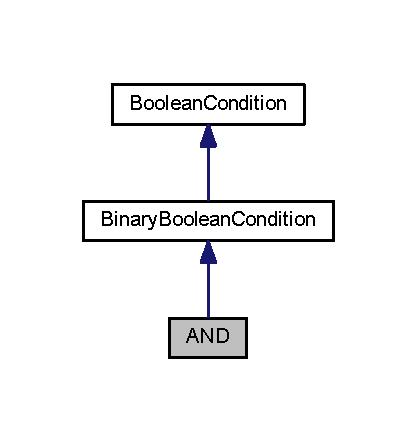
\includegraphics[width=200pt]{class_a_n_d__inherit__graph}
\end{center}
\end{figure}


Collaboration diagram for A\-N\-D\-:\nopagebreak
\begin{figure}[H]
\begin{center}
\leavevmode
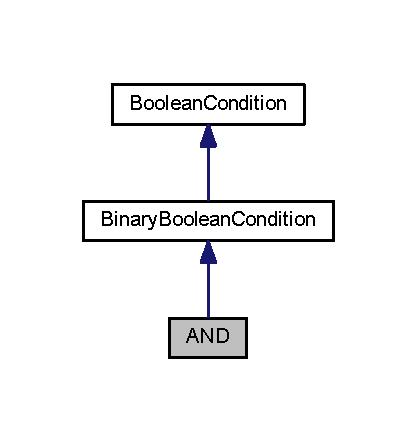
\includegraphics[width=200pt]{class_a_n_d__coll__graph}
\end{center}
\end{figure}
\subsection*{Public Member Functions}
\begin{DoxyCompactItemize}
\item 
\hyperlink{class_a_n_d_ac9edbd8cf77a985d900ff35828a02254}{A\-N\-D} (std\-::string body)
\begin{DoxyCompactList}\small\item\em Constructor. \end{DoxyCompactList}\item 
\hypertarget{class_a_n_d_a10556fbaba3e396f113b02bc5b3411c8}{virtual \hyperlink{class_a_n_d_a10556fbaba3e396f113b02bc5b3411c8}{$\sim$\-A\-N\-D} ()}\label{class_a_n_d_a10556fbaba3e396f113b02bc5b3411c8}

\begin{DoxyCompactList}\small\item\em Destructor. \end{DoxyCompactList}\item 
bool \hyperlink{class_a_n_d_af07972e6931b6800718ea88b160ef2d6}{eval} ()
\begin{DoxyCompactList}\small\item\em Evaluate the and combination. \end{DoxyCompactList}\end{DoxyCompactItemize}
\subsection*{Additional Inherited Members}


\subsection{Detailed Description}
And combination. 

\begin{DoxyAuthor}{Author}
David Lecoconnier 

Allan Mottier 
\end{DoxyAuthor}
\begin{DoxyDate}{Date}
2013-\/11-\/24 
\end{DoxyDate}


\subsection{Constructor \& Destructor Documentation}
\hypertarget{class_a_n_d_ac9edbd8cf77a985d900ff35828a02254}{\index{A\-N\-D@{A\-N\-D}!A\-N\-D@{A\-N\-D}}
\index{A\-N\-D@{A\-N\-D}!AND@{A\-N\-D}}
\subsubsection[{A\-N\-D}]{\setlength{\rightskip}{0pt plus 5cm}A\-N\-D\-::\-A\-N\-D (
\begin{DoxyParamCaption}
\item[{std\-::string}]{body}
\end{DoxyParamCaption}
)}}\label{class_a_n_d_ac9edbd8cf77a985d900ff35828a02254}


Constructor. 


\begin{DoxyParams}{Parameters}
{\em body} & text contained in I\-F structure \\
\hline
\end{DoxyParams}


\subsection{Member Function Documentation}
\hypertarget{class_a_n_d_af07972e6931b6800718ea88b160ef2d6}{\index{A\-N\-D@{A\-N\-D}!eval@{eval}}
\index{eval@{eval}!AND@{A\-N\-D}}
\subsubsection[{eval}]{\setlength{\rightskip}{0pt plus 5cm}bool A\-N\-D\-::eval (
\begin{DoxyParamCaption}
{}
\end{DoxyParamCaption}
)\hspace{0.3cm}{\ttfamily [virtual]}}}\label{class_a_n_d_af07972e6931b6800718ea88b160ef2d6}


Evaluate the and combination. 

\begin{DoxyReturn}{Returns}
true if combination is true 
\end{DoxyReturn}


Implements \hyperlink{class_boolean_condition}{Boolean\-Condition}.



The documentation for this class was generated from the following files\-:\begin{DoxyCompactItemize}
\item 
include/\-Booleans/A\-N\-D.\-h\item 
src/\-Booleans/A\-N\-D.\-cpp\end{DoxyCompactItemize}

\hypertarget{class_binary_boolean_condition}{\section{Binary\-Boolean\-Condition Class Reference}
\label{class_binary_boolean_condition}\index{Binary\-Boolean\-Condition@{Binary\-Boolean\-Condition}}
}


Represents a binary boolean condition. It contains two members.  




Inheritance diagram for Binary\-Boolean\-Condition\-:\nopagebreak
\begin{figure}[H]
\begin{center}
\leavevmode
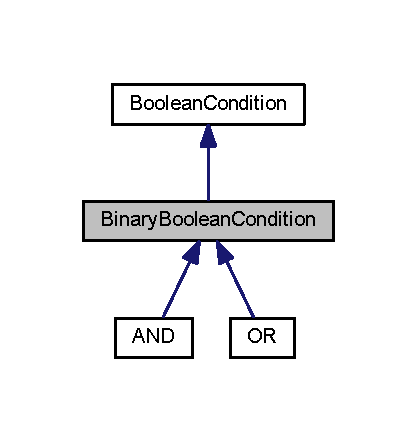
\includegraphics[width=200pt]{class_binary_boolean_condition__inherit__graph}
\end{center}
\end{figure}


Collaboration diagram for Binary\-Boolean\-Condition\-:\nopagebreak
\begin{figure}[H]
\begin{center}
\leavevmode
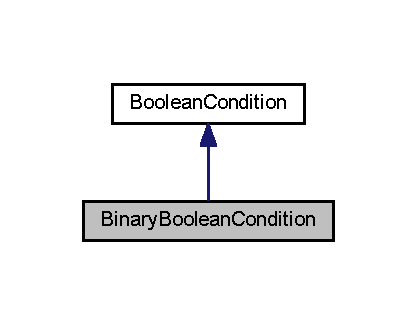
\includegraphics[width=200pt]{class_binary_boolean_condition__coll__graph}
\end{center}
\end{figure}
\subsection*{Public Member Functions}
\begin{DoxyCompactItemize}
\item 
\hyperlink{class_binary_boolean_condition_aaa28d7eee48ae1fa96944310a715962c}{Binary\-Boolean\-Condition} (std\-::string body)
\begin{DoxyCompactList}\small\item\em Constructor. \end{DoxyCompactList}\item 
\hypertarget{class_binary_boolean_condition_aa54534f1033d6cc84591a1dac7a99e76}{virtual \hyperlink{class_binary_boolean_condition_aa54534f1033d6cc84591a1dac7a99e76}{$\sim$\-Binary\-Boolean\-Condition} ()}\label{class_binary_boolean_condition_aa54534f1033d6cc84591a1dac7a99e76}

\begin{DoxyCompactList}\small\item\em Destructor. \end{DoxyCompactList}\item 
virtual \hyperlink{class_boolean_condition}{Boolean\-Condition} $\ast$ \hyperlink{class_binary_boolean_condition_ada259076d258bd3b7a50a66c42850923}{get\-Left} ()
\begin{DoxyCompactList}\small\item\em Return left part of the condition. \end{DoxyCompactList}\item 
virtual \hyperlink{class_boolean_condition}{Boolean\-Condition} $\ast$ \hyperlink{class_binary_boolean_condition_a5a35cf6749d7a7408fbef2b7229b53b3}{get\-Right} ()
\begin{DoxyCompactList}\small\item\em Return right part of the condition. \end{DoxyCompactList}\item 
virtual void \hyperlink{class_binary_boolean_condition_a3b7bc5b83b6ae0036bc14aae0f649b2f}{set\-Left} (\hyperlink{class_boolean_condition}{Boolean\-Condition} $\ast$bcond)
\begin{DoxyCompactList}\small\item\em Modify left part. \end{DoxyCompactList}\item 
virtual void \hyperlink{class_binary_boolean_condition_ad6902b875aca001608438fbc7e3143ff}{set\-Right} (\hyperlink{class_boolean_condition}{Boolean\-Condition} $\ast$bcond)
\begin{DoxyCompactList}\small\item\em Modify right part. \end{DoxyCompactList}\end{DoxyCompactItemize}
\subsection*{Additional Inherited Members}


\subsection{Detailed Description}
Represents a binary boolean condition. It contains two members. 

\begin{DoxyAuthor}{Author}
David Lecoconnier 

Allan Mottier 
\end{DoxyAuthor}
\begin{DoxyDate}{Date}
2013-\/11-\/24 
\end{DoxyDate}


\subsection{Constructor \& Destructor Documentation}
\hypertarget{class_binary_boolean_condition_aaa28d7eee48ae1fa96944310a715962c}{\index{Binary\-Boolean\-Condition@{Binary\-Boolean\-Condition}!Binary\-Boolean\-Condition@{Binary\-Boolean\-Condition}}
\index{Binary\-Boolean\-Condition@{Binary\-Boolean\-Condition}!BinaryBooleanCondition@{Binary\-Boolean\-Condition}}
\subsubsection[{Binary\-Boolean\-Condition}]{\setlength{\rightskip}{0pt plus 5cm}Binary\-Boolean\-Condition\-::\-Binary\-Boolean\-Condition (
\begin{DoxyParamCaption}
\item[{std\-::string}]{body}
\end{DoxyParamCaption}
)}}\label{class_binary_boolean_condition_aaa28d7eee48ae1fa96944310a715962c}


Constructor. 


\begin{DoxyParams}{Parameters}
{\em body} & text contained \\
\hline
\end{DoxyParams}


\subsection{Member Function Documentation}
\hypertarget{class_binary_boolean_condition_ada259076d258bd3b7a50a66c42850923}{\index{Binary\-Boolean\-Condition@{Binary\-Boolean\-Condition}!get\-Left@{get\-Left}}
\index{get\-Left@{get\-Left}!BinaryBooleanCondition@{Binary\-Boolean\-Condition}}
\subsubsection[{get\-Left}]{\setlength{\rightskip}{0pt plus 5cm}{\bf Boolean\-Condition} $\ast$ Binary\-Boolean\-Condition\-::get\-Left (
\begin{DoxyParamCaption}
{}
\end{DoxyParamCaption}
)\hspace{0.3cm}{\ttfamily [virtual]}}}\label{class_binary_boolean_condition_ada259076d258bd3b7a50a66c42850923}


Return left part of the condition. 

\begin{DoxyReturn}{Returns}
left part 
\end{DoxyReturn}
\hypertarget{class_binary_boolean_condition_a5a35cf6749d7a7408fbef2b7229b53b3}{\index{Binary\-Boolean\-Condition@{Binary\-Boolean\-Condition}!get\-Right@{get\-Right}}
\index{get\-Right@{get\-Right}!BinaryBooleanCondition@{Binary\-Boolean\-Condition}}
\subsubsection[{get\-Right}]{\setlength{\rightskip}{0pt plus 5cm}{\bf Boolean\-Condition} $\ast$ Binary\-Boolean\-Condition\-::get\-Right (
\begin{DoxyParamCaption}
{}
\end{DoxyParamCaption}
)\hspace{0.3cm}{\ttfamily [virtual]}}}\label{class_binary_boolean_condition_a5a35cf6749d7a7408fbef2b7229b53b3}


Return right part of the condition. 

\begin{DoxyReturn}{Returns}
right part 
\end{DoxyReturn}
\hypertarget{class_binary_boolean_condition_a3b7bc5b83b6ae0036bc14aae0f649b2f}{\index{Binary\-Boolean\-Condition@{Binary\-Boolean\-Condition}!set\-Left@{set\-Left}}
\index{set\-Left@{set\-Left}!BinaryBooleanCondition@{Binary\-Boolean\-Condition}}
\subsubsection[{set\-Left}]{\setlength{\rightskip}{0pt plus 5cm}void Binary\-Boolean\-Condition\-::set\-Left (
\begin{DoxyParamCaption}
\item[{{\bf Boolean\-Condition} $\ast$}]{bcond}
\end{DoxyParamCaption}
)\hspace{0.3cm}{\ttfamily [virtual]}}}\label{class_binary_boolean_condition_a3b7bc5b83b6ae0036bc14aae0f649b2f}


Modify left part. 


\begin{DoxyParams}{Parameters}
{\em bond} & a boolean condition \\
\hline
\end{DoxyParams}
\hypertarget{class_binary_boolean_condition_ad6902b875aca001608438fbc7e3143ff}{\index{Binary\-Boolean\-Condition@{Binary\-Boolean\-Condition}!set\-Right@{set\-Right}}
\index{set\-Right@{set\-Right}!BinaryBooleanCondition@{Binary\-Boolean\-Condition}}
\subsubsection[{set\-Right}]{\setlength{\rightskip}{0pt plus 5cm}void Binary\-Boolean\-Condition\-::set\-Right (
\begin{DoxyParamCaption}
\item[{{\bf Boolean\-Condition} $\ast$}]{bcond}
\end{DoxyParamCaption}
)\hspace{0.3cm}{\ttfamily [virtual]}}}\label{class_binary_boolean_condition_ad6902b875aca001608438fbc7e3143ff}


Modify right part. 


\begin{DoxyParams}{Parameters}
{\em bond} & a boolean condition \\
\hline
\end{DoxyParams}


The documentation for this class was generated from the following files\-:\begin{DoxyCompactItemize}
\item 
include/\-Booleans/Binary\-Boolean\-Condition.\-h\item 
src/\-Booleans/Binary\-Boolean\-Condition.\-cpp\end{DoxyCompactItemize}

\hypertarget{class_binary_number_condition}{\section{Binary\-Number\-Condition Class Reference}
\label{class_binary_number_condition}\index{Binary\-Number\-Condition@{Binary\-Number\-Condition}}
}


Represents a boolean condition in whiwh each member is numeral.  




Inheritance diagram for Binary\-Number\-Condition\-:\nopagebreak
\begin{figure}[H]
\begin{center}
\leavevmode
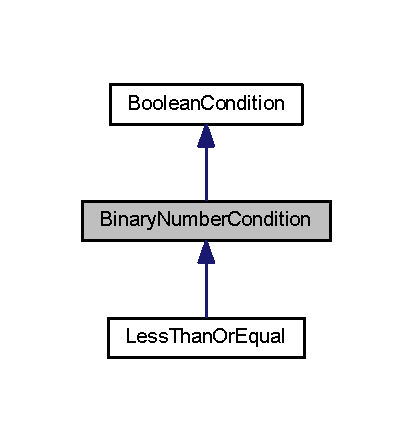
\includegraphics[width=198pt]{class_binary_number_condition__inherit__graph}
\end{center}
\end{figure}


Collaboration diagram for Binary\-Number\-Condition\-:\nopagebreak
\begin{figure}[H]
\begin{center}
\leavevmode
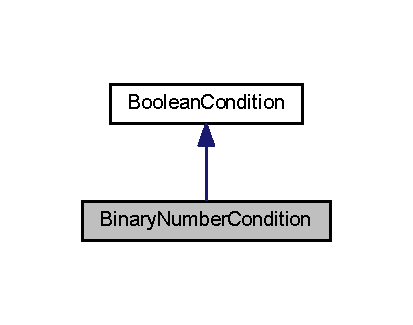
\includegraphics[width=198pt]{class_binary_number_condition__coll__graph}
\end{center}
\end{figure}
\subsection*{Public Member Functions}
\begin{DoxyCompactItemize}
\item 
\hyperlink{class_binary_number_condition_ab54fbec3be222a1574adb747090997a4}{Binary\-Number\-Condition} (std\-::string body)
\begin{DoxyCompactList}\small\item\em Constructor. \end{DoxyCompactList}\item 
\hypertarget{class_binary_number_condition_afe174df27a6314b89627912fe548428f}{virtual \hyperlink{class_binary_number_condition_afe174df27a6314b89627912fe548428f}{$\sim$\-Binary\-Number\-Condition} ()}\label{class_binary_number_condition_afe174df27a6314b89627912fe548428f}

\begin{DoxyCompactList}\small\item\em Destructor. \end{DoxyCompactList}\item 
virtual \hyperlink{class_expression}{Expression} $\ast$ \hyperlink{class_binary_number_condition_a903313505a12530fd277a1c5a2d9c77d}{get\-Left} ()
\begin{DoxyCompactList}\small\item\em Return left part of the condition. \end{DoxyCompactList}\item 
virtual \hyperlink{class_expression}{Expression} $\ast$ \hyperlink{class_binary_number_condition_a80dbf32cdd93d3bbccdc23ed0a9c0fc2}{get\-Right} ()
\begin{DoxyCompactList}\small\item\em Return right part of the condition. \end{DoxyCompactList}\item 
virtual void \hyperlink{class_binary_number_condition_a1e58428de3f4a63f08b6fc2be66abcac}{set\-Left} (\hyperlink{class_expression}{Expression} $\ast$expr)
\begin{DoxyCompactList}\small\item\em Modify left part. \end{DoxyCompactList}\item 
virtual void \hyperlink{class_binary_number_condition_a1b5978f5a31338ec72fd32e83e34c5fd}{set\-Right} (\hyperlink{class_expression}{Expression} $\ast$expr)
\begin{DoxyCompactList}\small\item\em Modify right part. \end{DoxyCompactList}\end{DoxyCompactItemize}
\subsection*{Additional Inherited Members}


\subsection{Detailed Description}
Represents a boolean condition in whiwh each member is numeral. 

\begin{DoxyAuthor}{Author}
David Lecoconnier 

Allan Mottier 
\end{DoxyAuthor}
\begin{DoxyDate}{Date}
2013-\/11-\/24 
\end{DoxyDate}


\subsection{Constructor \& Destructor Documentation}
\hypertarget{class_binary_number_condition_ab54fbec3be222a1574adb747090997a4}{\index{Binary\-Number\-Condition@{Binary\-Number\-Condition}!Binary\-Number\-Condition@{Binary\-Number\-Condition}}
\index{Binary\-Number\-Condition@{Binary\-Number\-Condition}!BinaryNumberCondition@{Binary\-Number\-Condition}}
\subsubsection[{Binary\-Number\-Condition}]{\setlength{\rightskip}{0pt plus 5cm}Binary\-Number\-Condition\-::\-Binary\-Number\-Condition (
\begin{DoxyParamCaption}
\item[{std\-::string}]{body}
\end{DoxyParamCaption}
)}}\label{class_binary_number_condition_ab54fbec3be222a1574adb747090997a4}


Constructor. 


\begin{DoxyParams}{Parameters}
{\em body} & text contained \\
\hline
\end{DoxyParams}


\subsection{Member Function Documentation}
\hypertarget{class_binary_number_condition_a903313505a12530fd277a1c5a2d9c77d}{\index{Binary\-Number\-Condition@{Binary\-Number\-Condition}!get\-Left@{get\-Left}}
\index{get\-Left@{get\-Left}!BinaryNumberCondition@{Binary\-Number\-Condition}}
\subsubsection[{get\-Left}]{\setlength{\rightskip}{0pt plus 5cm}{\bf Expression} $\ast$ Binary\-Number\-Condition\-::get\-Left (
\begin{DoxyParamCaption}
{}
\end{DoxyParamCaption}
)\hspace{0.3cm}{\ttfamily [virtual]}}}\label{class_binary_number_condition_a903313505a12530fd277a1c5a2d9c77d}


Return left part of the condition. 

\begin{DoxyReturn}{Returns}
left part 
\end{DoxyReturn}
\hypertarget{class_binary_number_condition_a80dbf32cdd93d3bbccdc23ed0a9c0fc2}{\index{Binary\-Number\-Condition@{Binary\-Number\-Condition}!get\-Right@{get\-Right}}
\index{get\-Right@{get\-Right}!BinaryNumberCondition@{Binary\-Number\-Condition}}
\subsubsection[{get\-Right}]{\setlength{\rightskip}{0pt plus 5cm}{\bf Expression} $\ast$ Binary\-Number\-Condition\-::get\-Right (
\begin{DoxyParamCaption}
{}
\end{DoxyParamCaption}
)\hspace{0.3cm}{\ttfamily [virtual]}}}\label{class_binary_number_condition_a80dbf32cdd93d3bbccdc23ed0a9c0fc2}


Return right part of the condition. 

\begin{DoxyReturn}{Returns}
right part 
\end{DoxyReturn}
\hypertarget{class_binary_number_condition_a1e58428de3f4a63f08b6fc2be66abcac}{\index{Binary\-Number\-Condition@{Binary\-Number\-Condition}!set\-Left@{set\-Left}}
\index{set\-Left@{set\-Left}!BinaryNumberCondition@{Binary\-Number\-Condition}}
\subsubsection[{set\-Left}]{\setlength{\rightskip}{0pt plus 5cm}void Binary\-Number\-Condition\-::set\-Left (
\begin{DoxyParamCaption}
\item[{{\bf Expression} $\ast$}]{expr}
\end{DoxyParamCaption}
)\hspace{0.3cm}{\ttfamily [virtual]}}}\label{class_binary_number_condition_a1e58428de3f4a63f08b6fc2be66abcac}


Modify left part. 


\begin{DoxyParams}{Parameters}
{\em expr} & an expression (not boolean one) \\
\hline
\end{DoxyParams}
\hypertarget{class_binary_number_condition_a1b5978f5a31338ec72fd32e83e34c5fd}{\index{Binary\-Number\-Condition@{Binary\-Number\-Condition}!set\-Right@{set\-Right}}
\index{set\-Right@{set\-Right}!BinaryNumberCondition@{Binary\-Number\-Condition}}
\subsubsection[{set\-Right}]{\setlength{\rightskip}{0pt plus 5cm}void Binary\-Number\-Condition\-::set\-Right (
\begin{DoxyParamCaption}
\item[{{\bf Expression} $\ast$}]{expr}
\end{DoxyParamCaption}
)\hspace{0.3cm}{\ttfamily [virtual]}}}\label{class_binary_number_condition_a1b5978f5a31338ec72fd32e83e34c5fd}


Modify right part. 


\begin{DoxyParams}{Parameters}
{\em expr} & an expression (not boolean one) \\
\hline
\end{DoxyParams}


The documentation for this class was generated from the following files\-:\begin{DoxyCompactItemize}
\item 
include/\-Booleans/Binary\-Number\-Condition.\-h\item 
src/\-Booleans/Binary\-Number\-Condition.\-cpp\end{DoxyCompactItemize}

\hypertarget{class_boolean}{\section{Boolean Class Reference}
\label{class_boolean}\index{Boolean@{Boolean}}
}


Represents a boolean object (Necesssary for construction of A\-S\-T)  




Inheritance diagram for Boolean\-:\nopagebreak
\begin{figure}[H]
\begin{center}
\leavevmode
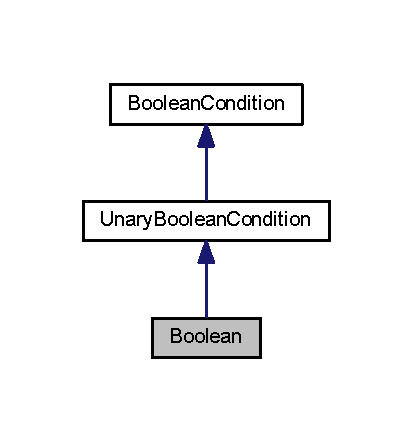
\includegraphics[width=198pt]{class_boolean__inherit__graph}
\end{center}
\end{figure}


Collaboration diagram for Boolean\-:\nopagebreak
\begin{figure}[H]
\begin{center}
\leavevmode
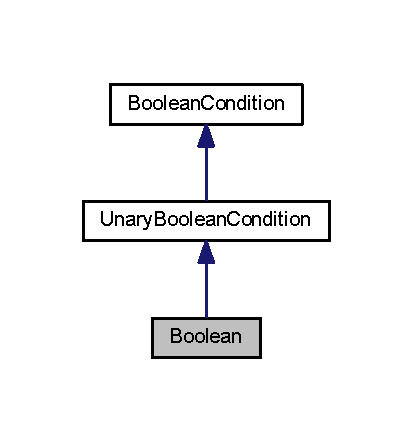
\includegraphics[width=198pt]{class_boolean__coll__graph}
\end{center}
\end{figure}
\subsection*{Public Member Functions}
\begin{DoxyCompactItemize}
\item 
\hyperlink{class_boolean_a3d0ffe778a52170ae7f4b7c9e2e80f9c}{Boolean} (bool val)
\begin{DoxyCompactList}\small\item\em Constructor. \end{DoxyCompactList}\item 
\hypertarget{class_boolean_a025bfd19cd093dbbe9492fdab16c056b}{virtual \hyperlink{class_boolean_a025bfd19cd093dbbe9492fdab16c056b}{$\sim$\-Boolean} ()}\label{class_boolean_a025bfd19cd093dbbe9492fdab16c056b}

\begin{DoxyCompactList}\small\item\em Destructor. \end{DoxyCompactList}\item 
\hypertarget{class_boolean_a18504725e866dbe8f1b9fcf5f19ee4dc}{virtual bool \hyperlink{class_boolean_a18504725e866dbe8f1b9fcf5f19ee4dc}{eval} ()}\label{class_boolean_a18504725e866dbe8f1b9fcf5f19ee4dc}

\begin{DoxyCompactList}\small\item\em Return the boolean value. \end{DoxyCompactList}\end{DoxyCompactItemize}
\subsection*{Protected Attributes}
\begin{DoxyCompactItemize}
\item 
\hypertarget{class_boolean_a900417114df9124e0398b926e2cb012d}{bool {\bfseries m\-\_\-val}}\label{class_boolean_a900417114df9124e0398b926e2cb012d}

\end{DoxyCompactItemize}
\subsection*{Additional Inherited Members}


\subsection{Detailed Description}
Represents a boolean object (Necesssary for construction of A\-S\-T) 

\begin{DoxyAuthor}{Author}
David Lecoconnier 

Allan Mottier 
\end{DoxyAuthor}
\begin{DoxyDate}{Date}
2013-\/11-\/24 
\end{DoxyDate}


\subsection{Constructor \& Destructor Documentation}
\hypertarget{class_boolean_a3d0ffe778a52170ae7f4b7c9e2e80f9c}{\index{Boolean@{Boolean}!Boolean@{Boolean}}
\index{Boolean@{Boolean}!Boolean@{Boolean}}
\subsubsection[{Boolean}]{\setlength{\rightskip}{0pt plus 5cm}Boolean\-::\-Boolean (
\begin{DoxyParamCaption}
\item[{bool}]{val}
\end{DoxyParamCaption}
)}}\label{class_boolean_a3d0ffe778a52170ae7f4b7c9e2e80f9c}


Constructor. 


\begin{DoxyParams}{Parameters}
{\em val} & a bool value \\
\hline
\end{DoxyParams}


The documentation for this class was generated from the following files\-:\begin{DoxyCompactItemize}
\item 
include/\-Booleans/Boolean.\-h\item 
src/\-Booleans/Boolean.\-cpp\end{DoxyCompactItemize}

\hypertarget{class_boolean_condition}{\section{Boolean\-Condition Class Reference}
\label{class_boolean_condition}\index{Boolean\-Condition@{Boolean\-Condition}}
}


Abstract boolean condition. It should be an expression but is is not to simplify calculus.  




Inheritance diagram for Boolean\-Condition\-:\nopagebreak
\begin{figure}[H]
\begin{center}
\leavevmode
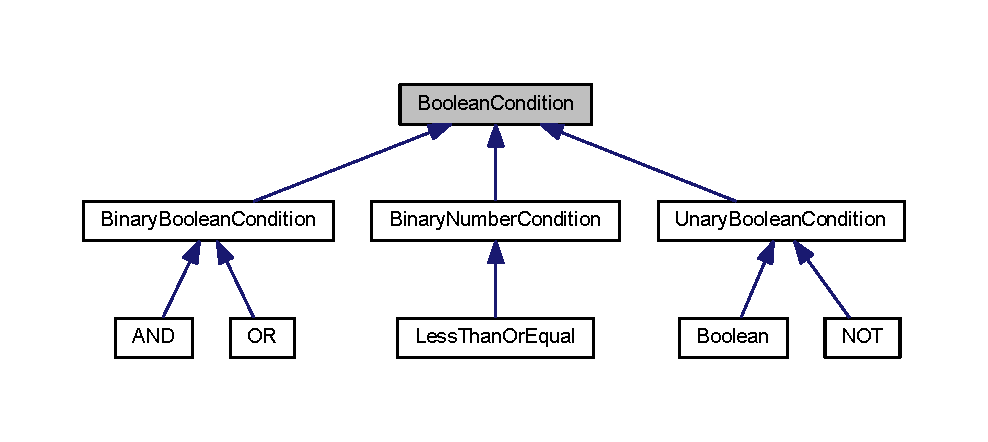
\includegraphics[width=350pt]{class_boolean_condition__inherit__graph}
\end{center}
\end{figure}
\subsection*{Public Member Functions}
\begin{DoxyCompactItemize}
\item 
\hyperlink{class_boolean_condition_a7566e4b7418a39def0a6f9f4a4c36d59}{Boolean\-Condition} (std\-::string body)
\begin{DoxyCompactList}\small\item\em Constructor. \end{DoxyCompactList}\item 
\hypertarget{class_boolean_condition_a93e485184e45ac484ba6dcff8ce837a5}{virtual \hyperlink{class_boolean_condition_a93e485184e45ac484ba6dcff8ce837a5}{$\sim$\-Boolean\-Condition} ()}\label{class_boolean_condition_a93e485184e45ac484ba6dcff8ce837a5}

\begin{DoxyCompactList}\small\item\em Destructor. \end{DoxyCompactList}\item 
\hypertarget{class_boolean_condition_a0aa5de22637022585f20c9254723406e}{virtual bool {\bfseries eval} ()=0}\label{class_boolean_condition_a0aa5de22637022585f20c9254723406e}

\end{DoxyCompactItemize}
\subsection*{Protected Member Functions}
\begin{DoxyCompactItemize}
\item 
void \hyperlink{class_boolean_condition_aefb27ea0d173870ff2e37b7e7ef8291b}{set\-Body} (std\-::string body)
\begin{DoxyCompactList}\small\item\em Modify body text. \end{DoxyCompactList}\item 
std\-::string \hyperlink{class_boolean_condition_ae8dba5559c11a5781a41a9ec69e7feaf}{get\-Body} ()
\begin{DoxyCompactList}\small\item\em Return body text. \end{DoxyCompactList}\end{DoxyCompactItemize}


\subsection{Detailed Description}
Abstract boolean condition. It should be an expression but is is not to simplify calculus. 

\begin{DoxyAuthor}{Author}
David Lecoconnier 

Allan Mottier 
\end{DoxyAuthor}
\begin{DoxyDate}{Date}
2013-\/11-\/24 
\end{DoxyDate}


\subsection{Constructor \& Destructor Documentation}
\hypertarget{class_boolean_condition_a7566e4b7418a39def0a6f9f4a4c36d59}{\index{Boolean\-Condition@{Boolean\-Condition}!Boolean\-Condition@{Boolean\-Condition}}
\index{Boolean\-Condition@{Boolean\-Condition}!BooleanCondition@{Boolean\-Condition}}
\subsubsection[{Boolean\-Condition}]{\setlength{\rightskip}{0pt plus 5cm}Boolean\-Condition\-::\-Boolean\-Condition (
\begin{DoxyParamCaption}
\item[{std\-::string}]{body}
\end{DoxyParamCaption}
)}}\label{class_boolean_condition_a7566e4b7418a39def0a6f9f4a4c36d59}


Constructor. 


\begin{DoxyParams}{Parameters}
{\em body} & text \\
\hline
\end{DoxyParams}


\subsection{Member Function Documentation}
\hypertarget{class_boolean_condition_ae8dba5559c11a5781a41a9ec69e7feaf}{\index{Boolean\-Condition@{Boolean\-Condition}!get\-Body@{get\-Body}}
\index{get\-Body@{get\-Body}!BooleanCondition@{Boolean\-Condition}}
\subsubsection[{get\-Body}]{\setlength{\rightskip}{0pt plus 5cm}std\-::string Boolean\-Condition\-::get\-Body (
\begin{DoxyParamCaption}
{}
\end{DoxyParamCaption}
)\hspace{0.3cm}{\ttfamily [protected]}}}\label{class_boolean_condition_ae8dba5559c11a5781a41a9ec69e7feaf}


Return body text. 

\begin{DoxyReturn}{Returns}
text 
\end{DoxyReturn}
\hypertarget{class_boolean_condition_aefb27ea0d173870ff2e37b7e7ef8291b}{\index{Boolean\-Condition@{Boolean\-Condition}!set\-Body@{set\-Body}}
\index{set\-Body@{set\-Body}!BooleanCondition@{Boolean\-Condition}}
\subsubsection[{set\-Body}]{\setlength{\rightskip}{0pt plus 5cm}void Boolean\-Condition\-::set\-Body (
\begin{DoxyParamCaption}
\item[{std\-::string}]{body}
\end{DoxyParamCaption}
)\hspace{0.3cm}{\ttfamily [protected]}}}\label{class_boolean_condition_aefb27ea0d173870ff2e37b7e7ef8291b}


Modify body text. 


\begin{DoxyParams}{Parameters}
{\em body} & body text \\
\hline
\end{DoxyParams}


The documentation for this class was generated from the following files\-:\begin{DoxyCompactItemize}
\item 
include/\-Booleans/Boolean\-Condition.\-h\item 
src/\-Booleans/Boolean\-Condition.\-cpp\end{DoxyCompactItemize}

\hypertarget{class_context}{\section{Context Class Reference}
\label{class_context}\index{Context@{Context}}
}


A context is a mix between the stack and the heap in which variables are stored.  




Inheritance diagram for Context\-:\nopagebreak
\begin{figure}[H]
\begin{center}
\leavevmode
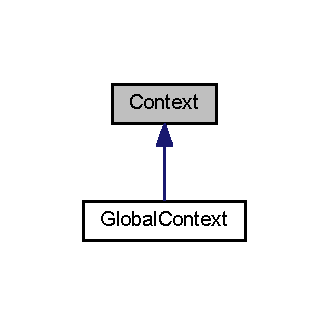
\includegraphics[width=158pt]{class_context__inherit__graph}
\end{center}
\end{figure}


Collaboration diagram for Context\-:\nopagebreak
\begin{figure}[H]
\begin{center}
\leavevmode
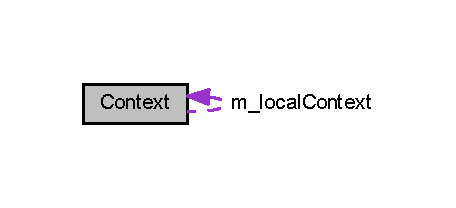
\includegraphics[width=219pt]{class_context__coll__graph}
\end{center}
\end{figure}
\subsection*{Public Member Functions}
\begin{DoxyCompactItemize}
\item 
\hypertarget{class_context_a652cdcd2eedc8dbd9110bd284c5d5cf0}{\hyperlink{class_context_a652cdcd2eedc8dbd9110bd284c5d5cf0}{Context} ()}\label{class_context_a652cdcd2eedc8dbd9110bd284c5d5cf0}

\begin{DoxyCompactList}\small\item\em Constructor. \end{DoxyCompactList}\item 
\hypertarget{class_context_a2d34e4556448e40693f61d15e091b604}{\hyperlink{class_context_a2d34e4556448e40693f61d15e091b604}{$\sim$\-Context} ()}\label{class_context_a2d34e4556448e40693f61d15e091b604}

\begin{DoxyCompactList}\small\item\em Destructor. \end{DoxyCompactList}\item 
bool \hyperlink{class_context_a749420a035d008bb388fb2d737f973b0}{delete\-Last\-Local\-Context} ()
\begin{DoxyCompactList}\small\item\em Remove the youngest context. \end{DoxyCompactList}\item 
\hypertarget{class_context_a06fd882c9625b60a6130ab1e4537e38e}{void \hyperlink{class_context_a06fd882c9625b60a6130ab1e4537e38e}{add\-New\-Local\-Contest} ()}\label{class_context_a06fd882c9625b60a6130ab1e4537e38e}

\begin{DoxyCompactList}\small\item\em Create a new context. \end{DoxyCompactList}\item 
void \hyperlink{class_context_a0923de09c4e6e42ba5ab96ca961af86b}{add\-New\-Variable\-In\-Last\-Context} (std\-::string name, \hyperlink{class_number}{Number} $\ast$number)
\begin{DoxyCompactList}\small\item\em \hyperlink{class_add}{Add} a new variable in the youngest context. \end{DoxyCompactList}\item 
bool \hyperlink{class_context_a00cf96423533f26bf1457f181e47a885}{modify} (std\-::string name, \hyperlink{class_number}{Number} $\ast$number)
\begin{DoxyCompactList}\small\item\em Modify the value of a variable in the youngest context. \end{DoxyCompactList}\item 
bool \hyperlink{class_context_a4e5513c1557b91b9ba4897ca6239e664}{is\-Containing} (std\-::string name)
\begin{DoxyCompactList}\small\item\em Test the presence of a variable in contexts. \end{DoxyCompactList}\item 
\hyperlink{class_number}{Number} $\ast$ \hyperlink{class_context_a0924ac4b20a004cc5d87b0b360111832}{get\-Number} (std\-::string name)
\begin{DoxyCompactList}\small\item\em Return the youngest \hyperlink{class_number}{Number} of a variable. \end{DoxyCompactList}\end{DoxyCompactItemize}
\subsection*{Protected Member Functions}
\begin{DoxyCompactItemize}
\item 
bool \hyperlink{class_context_a84b15fffee0ce1176cb995122f0573b9}{has\-Next\-Local\-Context} ()
\begin{DoxyCompactList}\small\item\em Test if there is a next context. \end{DoxyCompactList}\end{DoxyCompactItemize}
\subsection*{Protected Attributes}
\begin{DoxyCompactItemize}
\item 
\hypertarget{class_context_aa3a6edbb214af148252961f74d3fa4f1}{\hyperlink{class_context}{Context} $\ast$ {\bfseries m\-\_\-local\-Context}}\label{class_context_aa3a6edbb214af148252961f74d3fa4f1}

\item 
\hypertarget{class_context_a80bc700bd57760f144c5ac9e2175a287}{std\-::map$<$ std\-::string, \hyperlink{class_number}{Number} $>$ $\ast$ {\bfseries m\-\_\-map}}\label{class_context_a80bc700bd57760f144c5ac9e2175a287}

\end{DoxyCompactItemize}


\subsection{Detailed Description}
A context is a mix between the stack and the heap in which variables are stored. 

\begin{DoxyAuthor}{Author}
David Lecoconnier 

Allan Mottier 
\end{DoxyAuthor}
\begin{DoxyDate}{Date}
2013-\/11-\/24 
\end{DoxyDate}


\subsection{Member Function Documentation}
\hypertarget{class_context_a0923de09c4e6e42ba5ab96ca961af86b}{\index{Context@{Context}!add\-New\-Variable\-In\-Last\-Context@{add\-New\-Variable\-In\-Last\-Context}}
\index{add\-New\-Variable\-In\-Last\-Context@{add\-New\-Variable\-In\-Last\-Context}!Context@{Context}}
\subsubsection[{add\-New\-Variable\-In\-Last\-Context}]{\setlength{\rightskip}{0pt plus 5cm}void Context\-::add\-New\-Variable\-In\-Last\-Context (
\begin{DoxyParamCaption}
\item[{std\-::string}]{name, }
\item[{{\bf Number} $\ast$}]{number}
\end{DoxyParamCaption}
)}}\label{class_context_a0923de09c4e6e42ba5ab96ca961af86b}


\hyperlink{class_add}{Add} a new variable in the youngest context. 


\begin{DoxyParams}{Parameters}
{\em name} & variable's name \\
\hline
{\em number} & variable's value \\
\hline
\end{DoxyParams}
\hypertarget{class_context_a749420a035d008bb388fb2d737f973b0}{\index{Context@{Context}!delete\-Last\-Local\-Context@{delete\-Last\-Local\-Context}}
\index{delete\-Last\-Local\-Context@{delete\-Last\-Local\-Context}!Context@{Context}}
\subsubsection[{delete\-Last\-Local\-Context}]{\setlength{\rightskip}{0pt plus 5cm}bool Context\-::delete\-Last\-Local\-Context (
\begin{DoxyParamCaption}
{}
\end{DoxyParamCaption}
)}}\label{class_context_a749420a035d008bb388fb2d737f973b0}


Remove the youngest context. 

\begin{DoxyReturn}{Returns}
true on success 
\end{DoxyReturn}
\hypertarget{class_context_a0924ac4b20a004cc5d87b0b360111832}{\index{Context@{Context}!get\-Number@{get\-Number}}
\index{get\-Number@{get\-Number}!Context@{Context}}
\subsubsection[{get\-Number}]{\setlength{\rightskip}{0pt plus 5cm}{\bf Number} $\ast$ Context\-::get\-Number (
\begin{DoxyParamCaption}
\item[{std\-::string}]{name}
\end{DoxyParamCaption}
)}}\label{class_context_a0924ac4b20a004cc5d87b0b360111832}


Return the youngest \hyperlink{class_number}{Number} of a variable. 


\begin{DoxyParams}{Parameters}
{\em name} & variable's name \\
\hline
\end{DoxyParams}
\begin{DoxyReturn}{Returns}
the variable's value 
\end{DoxyReturn}
\hypertarget{class_context_a84b15fffee0ce1176cb995122f0573b9}{\index{Context@{Context}!has\-Next\-Local\-Context@{has\-Next\-Local\-Context}}
\index{has\-Next\-Local\-Context@{has\-Next\-Local\-Context}!Context@{Context}}
\subsubsection[{has\-Next\-Local\-Context}]{\setlength{\rightskip}{0pt plus 5cm}bool Context\-::has\-Next\-Local\-Context (
\begin{DoxyParamCaption}
{}
\end{DoxyParamCaption}
)\hspace{0.3cm}{\ttfamily [protected]}}}\label{class_context_a84b15fffee0ce1176cb995122f0573b9}


Test if there is a next context. 

\begin{DoxyReturn}{Returns}
true if present 
\end{DoxyReturn}
\hypertarget{class_context_a4e5513c1557b91b9ba4897ca6239e664}{\index{Context@{Context}!is\-Containing@{is\-Containing}}
\index{is\-Containing@{is\-Containing}!Context@{Context}}
\subsubsection[{is\-Containing}]{\setlength{\rightskip}{0pt plus 5cm}bool Context\-::is\-Containing (
\begin{DoxyParamCaption}
\item[{std\-::string}]{name}
\end{DoxyParamCaption}
)}}\label{class_context_a4e5513c1557b91b9ba4897ca6239e664}


Test the presence of a variable in contexts. 


\begin{DoxyParams}{Parameters}
{\em name} & variable's name \\
\hline
\end{DoxyParams}
\begin{DoxyReturn}{Returns}
true if present 
\end{DoxyReturn}
\hypertarget{class_context_a00cf96423533f26bf1457f181e47a885}{\index{Context@{Context}!modify@{modify}}
\index{modify@{modify}!Context@{Context}}
\subsubsection[{modify}]{\setlength{\rightskip}{0pt plus 5cm}bool Context\-::modify (
\begin{DoxyParamCaption}
\item[{std\-::string}]{name, }
\item[{{\bf Number} $\ast$}]{number}
\end{DoxyParamCaption}
)}}\label{class_context_a00cf96423533f26bf1457f181e47a885}


Modify the value of a variable in the youngest context. 


\begin{DoxyParams}{Parameters}
{\em name} & variable's name \\
\hline
{\em number} & variable's value \\
\hline
\end{DoxyParams}
\begin{DoxyReturn}{Returns}
true on success 
\end{DoxyReturn}


The documentation for this class was generated from the following files\-:\begin{DoxyCompactItemize}
\item 
include/\-Memory/Context.\-h\item 
src/\-Memory/Context.\-cpp\end{DoxyCompactItemize}

\hypertarget{class_divide}{\section{Divide Class Reference}
\label{class_divide}\index{Divide@{Divide}}
}


\hyperlink{class_divide}{Divide} operation.  




Inheritance diagram for Divide\-:\nopagebreak
\begin{figure}[H]
\begin{center}
\leavevmode
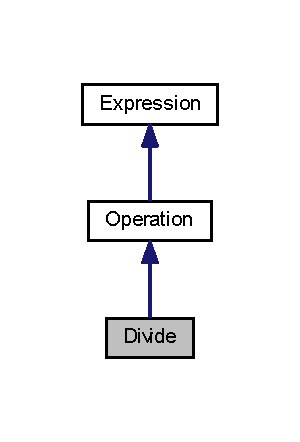
\includegraphics[width=144pt]{class_divide__inherit__graph}
\end{center}
\end{figure}


Collaboration diagram for Divide\-:\nopagebreak
\begin{figure}[H]
\begin{center}
\leavevmode
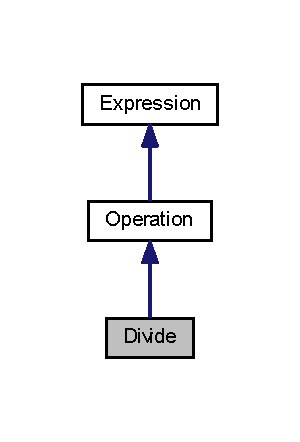
\includegraphics[width=144pt]{class_divide__coll__graph}
\end{center}
\end{figure}
\subsection*{Public Member Functions}
\begin{DoxyCompactItemize}
\item 
\hyperlink{class_divide_aced11d56b3d236557054bd066309dd82}{Divide} (std\-::string body)
\begin{DoxyCompactList}\small\item\em Default constructor. \end{DoxyCompactList}\item 
virtual \hyperlink{class_divide_a10ccbd35f5d37bdb2fe66988db462e06}{$\sim$\-Divide} ()
\begin{DoxyCompactList}\small\item\em Default destructor. \end{DoxyCompactList}\item 
virtual \hyperlink{class_abstract_number}{Abstract\-Number} $\ast$ \hyperlink{class_divide_ac4042774f748a5af09d2091a1d281195}{eval} (std\-::list$<$ \hyperlink{class_expression}{Expression} $\ast$ $>$ $\ast$args)
\begin{DoxyCompactList}\small\item\em Evaluate the \hyperlink{class_divide}{Divide} operation. \end{DoxyCompactList}\end{DoxyCompactItemize}
\subsection*{Additional Inherited Members}


\subsection{Detailed Description}
\hyperlink{class_divide}{Divide} operation. 

\begin{DoxyAuthor}{Author}
David Lecoconnier 

Allan Mottier 
\end{DoxyAuthor}
\begin{DoxyDate}{Date}
2013-\/11-\/24 
\end{DoxyDate}


\subsection{Constructor \& Destructor Documentation}
\hypertarget{class_divide_aced11d56b3d236557054bd066309dd82}{\index{Divide@{Divide}!Divide@{Divide}}
\index{Divide@{Divide}!Divide@{Divide}}
\subsubsection[{Divide}]{\setlength{\rightskip}{0pt plus 5cm}Divide\-::\-Divide (
\begin{DoxyParamCaption}
\item[{std\-::string}]{body}
\end{DoxyParamCaption}
)}}\label{class_divide_aced11d56b3d236557054bd066309dd82}


Default constructor. 

Constructor.


\begin{DoxyParams}{Parameters}
{\em body} & text contained \\
\hline
\end{DoxyParams}
\hypertarget{class_divide_a10ccbd35f5d37bdb2fe66988db462e06}{\index{Divide@{Divide}!$\sim$\-Divide@{$\sim$\-Divide}}
\index{$\sim$\-Divide@{$\sim$\-Divide}!Divide@{Divide}}
\subsubsection[{$\sim$\-Divide}]{\setlength{\rightskip}{0pt plus 5cm}Divide\-::$\sim$\-Divide (
\begin{DoxyParamCaption}
{}
\end{DoxyParamCaption}
)\hspace{0.3cm}{\ttfamily [virtual]}}}\label{class_divide_a10ccbd35f5d37bdb2fe66988db462e06}


Default destructor. 

Destructor. 

\subsection{Member Function Documentation}
\hypertarget{class_divide_ac4042774f748a5af09d2091a1d281195}{\index{Divide@{Divide}!eval@{eval}}
\index{eval@{eval}!Divide@{Divide}}
\subsubsection[{eval}]{\setlength{\rightskip}{0pt plus 5cm}{\bf Abstract\-Number} $\ast$ Divide\-::eval (
\begin{DoxyParamCaption}
\item[{std\-::list$<$ {\bf Expression} $\ast$ $>$ $\ast$}]{args}
\end{DoxyParamCaption}
)\hspace{0.3cm}{\ttfamily [virtual]}}}\label{class_divide_ac4042774f748a5af09d2091a1d281195}


Evaluate the \hyperlink{class_divide}{Divide} operation. 


\begin{DoxyParams}{Parameters}
{\em args} & -\/\-Useless-\/ \\
\hline
\end{DoxyParams}
\begin{DoxyReturn}{Returns}
the result 
\end{DoxyReturn}


Implements \hyperlink{class_expression}{Expression}.



The documentation for this class was generated from the following files\-:\begin{DoxyCompactItemize}
\item 
include/\-Numbers/Divide.\-h\item 
src/\-Numbers/Divide.\-cpp\end{DoxyCompactItemize}

\hypertarget{class_expression}{\section{Expression Class Reference}
\label{class_expression}\index{Expression@{Expression}}
}


Generalized representation of an expression.  




Inheritance diagram for Expression\-:\nopagebreak
\begin{figure}[H]
\begin{center}
\leavevmode
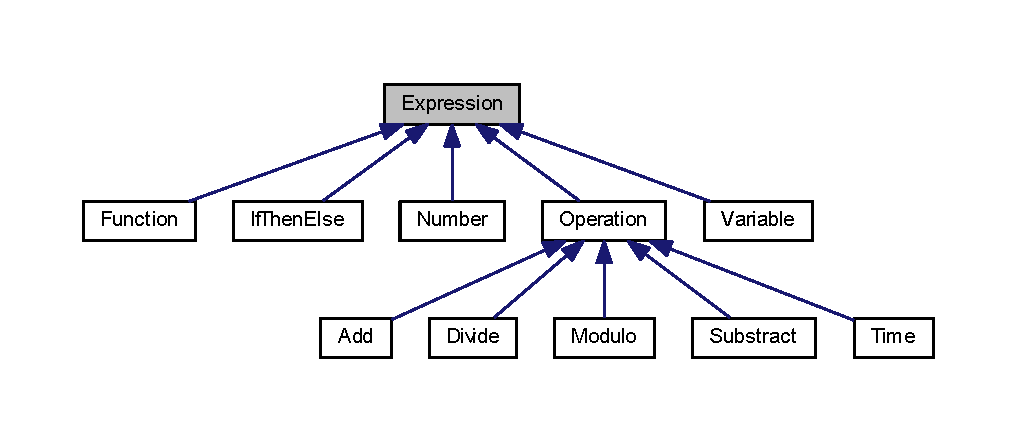
\includegraphics[width=350pt]{class_expression__inherit__graph}
\end{center}
\end{figure}
\subsection*{Public Member Functions}
\begin{DoxyCompactItemize}
\item 
\hyperlink{class_expression_a42980da61e3dab5edd4ef12ab10d047b}{Expression} (std\-::string body)
\begin{DoxyCompactList}\small\item\em Default constructor. \end{DoxyCompactList}\item 
virtual \hyperlink{class_expression_a3e99570b177da619eeb2c5787cbb148e}{$\sim$\-Expression} ()
\begin{DoxyCompactList}\small\item\em Default destructor. \end{DoxyCompactList}\item 
\hypertarget{class_expression_a5b20a3a102b7da3f53203b867859ba7c}{virtual \hyperlink{class_abstract_number}{Abstract\-Number} $\ast$ {\bfseries eval} (std\-::list$<$ \hyperlink{class_expression}{Expression} $\ast$ $>$ $\ast$args)=0}\label{class_expression_a5b20a3a102b7da3f53203b867859ba7c}

\item 
std\-::string \hyperlink{class_expression_a5c403d29fd47e5363ff70ee813a805f4}{get\-Body} ()
\begin{DoxyCompactList}\small\item\em Return the body text. \end{DoxyCompactList}\end{DoxyCompactItemize}
\subsection*{Protected Member Functions}
\begin{DoxyCompactItemize}
\item 
void \hyperlink{class_expression_a4889a8b18a6e996b78b87ed61a5f3595}{set\-Body} (std\-::string body)
\begin{DoxyCompactList}\small\item\em Modify the body text. \end{DoxyCompactList}\end{DoxyCompactItemize}


\subsection{Detailed Description}
Generalized representation of an expression. 

\begin{DoxyAuthor}{Author}
David Lecoconnier 

Allan Mottier 
\end{DoxyAuthor}
\begin{DoxyDate}{Date}
2013-\/11-\/24 
\end{DoxyDate}


\subsection{Constructor \& Destructor Documentation}
\hypertarget{class_expression_a42980da61e3dab5edd4ef12ab10d047b}{\index{Expression@{Expression}!Expression@{Expression}}
\index{Expression@{Expression}!Expression@{Expression}}
\subsubsection[{Expression}]{\setlength{\rightskip}{0pt plus 5cm}Expression\-::\-Expression (
\begin{DoxyParamCaption}
\item[{std\-::string}]{body}
\end{DoxyParamCaption}
)}}\label{class_expression_a42980da61e3dab5edd4ef12ab10d047b}


Default constructor. 

Constructor.


\begin{DoxyParams}{Parameters}
{\em body} & text contained \\
\hline
\end{DoxyParams}
\hypertarget{class_expression_a3e99570b177da619eeb2c5787cbb148e}{\index{Expression@{Expression}!$\sim$\-Expression@{$\sim$\-Expression}}
\index{$\sim$\-Expression@{$\sim$\-Expression}!Expression@{Expression}}
\subsubsection[{$\sim$\-Expression}]{\setlength{\rightskip}{0pt plus 5cm}Expression\-::$\sim$\-Expression (
\begin{DoxyParamCaption}
{}
\end{DoxyParamCaption}
)\hspace{0.3cm}{\ttfamily [virtual]}}}\label{class_expression_a3e99570b177da619eeb2c5787cbb148e}


Default destructor. 

Destructor. 

\subsection{Member Function Documentation}
\hypertarget{class_expression_a5c403d29fd47e5363ff70ee813a805f4}{\index{Expression@{Expression}!get\-Body@{get\-Body}}
\index{get\-Body@{get\-Body}!Expression@{Expression}}
\subsubsection[{get\-Body}]{\setlength{\rightskip}{0pt plus 5cm}std\-::string Expression\-::get\-Body (
\begin{DoxyParamCaption}
{}
\end{DoxyParamCaption}
)}}\label{class_expression_a5c403d29fd47e5363ff70ee813a805f4}


Return the body text. 

\begin{DoxyReturn}{Returns}
a string 
\end{DoxyReturn}
\hypertarget{class_expression_a4889a8b18a6e996b78b87ed61a5f3595}{\index{Expression@{Expression}!set\-Body@{set\-Body}}
\index{set\-Body@{set\-Body}!Expression@{Expression}}
\subsubsection[{set\-Body}]{\setlength{\rightskip}{0pt plus 5cm}void Expression\-::set\-Body (
\begin{DoxyParamCaption}
\item[{std\-::string}]{body}
\end{DoxyParamCaption}
)\hspace{0.3cm}{\ttfamily [protected]}}}\label{class_expression_a4889a8b18a6e996b78b87ed61a5f3595}


Modify the body text. 


\begin{DoxyParams}{Parameters}
{\em body} & a text \\
\hline
\end{DoxyParams}


The documentation for this class was generated from the following files\-:\begin{DoxyCompactItemize}
\item 
include/Expression.\-h\item 
src/Expression.\-cpp\end{DoxyCompactItemize}

\hypertarget{class_factory}{\section{Factory Class Reference}
\label{class_factory}\index{Factory@{Factory}}
}


\hyperlink{class_factory}{Factory} for creation of all part of the A\-S\-T.  




{\ttfamily \#include $<$index\-H\-T\-M\-Lpage.\-h$>$}

\subsection*{Static Public Member Functions}
\begin{DoxyCompactItemize}
\item 
\hypertarget{class_factory_aab7c0825e04728bfa9b515a6ddd6e48f}{static \hyperlink{class_operation}{Operation} $\ast$ {\bfseries create\-Add\-Operation} (std\-::string body)}\label{class_factory_aab7c0825e04728bfa9b515a6ddd6e48f}

\item 
\hypertarget{class_factory_aa75e36275f769c48e55ef0740af5ddbc}{static \hyperlink{class_operation}{Operation} $\ast$ {\bfseries create\-Divide\-Operation} (std\-::string body)}\label{class_factory_aa75e36275f769c48e55ef0740af5ddbc}

\item 
\hypertarget{class_factory_afb9cf1ac84a9275ce0d3d68cae883266}{static \hyperlink{class_operation}{Operation} $\ast$ {\bfseries create\-Modulo\-Operation} (std\-::string body)}\label{class_factory_afb9cf1ac84a9275ce0d3d68cae883266}

\item 
\hypertarget{class_factory_a4061f85223d97fc151ec35b8644eae3a}{static \hyperlink{class_operation}{Operation} $\ast$ {\bfseries create\-Substract\-Operation} (std\-::string body)}\label{class_factory_a4061f85223d97fc151ec35b8644eae3a}

\item 
\hypertarget{class_factory_ac80521d608a2c985391558c781aba2e4}{static \hyperlink{class_operation}{Operation} $\ast$ {\bfseries create\-Time\-Operation} (std\-::string body)}\label{class_factory_ac80521d608a2c985391558c781aba2e4}

\item 
\hypertarget{class_factory_a4a66797d735b0b0d9e37fee865fe6f43}{static \hyperlink{class_number}{Number} $\ast$ {\bfseries create\-Integer\-Number} (int val)}\label{class_factory_a4a66797d735b0b0d9e37fee865fe6f43}

\item 
\hypertarget{class_factory_a63257c7056b6a95ffabeba379cb91bf9}{static \hyperlink{class_number}{Number} $\ast$ {\bfseries create\-Real\-Number} (float val)}\label{class_factory_a63257c7056b6a95ffabeba379cb91bf9}

\item 
\hypertarget{class_factory_afe22780981f76f177804f606f43f9699}{static \hyperlink{class_number}{Number} $\ast$ {\bfseries create\-Number} (std\-::string val)}\label{class_factory_afe22780981f76f177804f606f43f9699}

\item 
\hypertarget{class_factory_a2618c1e3fe60d0c95e065eb31cf4c165}{static \hyperlink{class_context}{Context} $\ast$ {\bfseries create\-New\-Local\-Context} ()}\label{class_factory_a2618c1e3fe60d0c95e065eb31cf4c165}

\item 
\hypertarget{class_factory_a787e45866dd2dcadd4623ebea9bff41e}{static \hyperlink{class_binary_boolean_condition}{Binary\-Boolean\-Condition} $\ast$ {\bfseries create\-New\-A\-N\-D\-Operation} (std\-::string body)}\label{class_factory_a787e45866dd2dcadd4623ebea9bff41e}

\item 
\hypertarget{class_factory_a6b9e1d0c972e9c50c21d289c3539a8cb}{static \hyperlink{class_binary_boolean_condition}{Binary\-Boolean\-Condition} $\ast$ {\bfseries create\-New\-O\-R\-Operation} (std\-::string body)}\label{class_factory_a6b9e1d0c972e9c50c21d289c3539a8cb}

\item 
\hypertarget{class_factory_ab66c0668a22c434167cf2304d2fd2f5d}{static \hyperlink{class_unary_boolean_condition}{Unary\-Boolean\-Condition} $\ast$ {\bfseries create\-New\-N\-O\-T\-Operation} (std\-::string body)}\label{class_factory_ab66c0668a22c434167cf2304d2fd2f5d}

\item 
\hypertarget{class_factory_a829f2144264e2a42ad2262d17dc2d89d}{static \hyperlink{class_unary_boolean_condition}{Unary\-Boolean\-Condition} $\ast$ {\bfseries create\-New\-Boolean} (bool val)}\label{class_factory_a829f2144264e2a42ad2262d17dc2d89d}

\item 
\hypertarget{class_factory_a2b3007496f889a25ec1a4e7f44f2c156}{static \hyperlink{class_binary_number_condition}{Binary\-Number\-Condition} $\ast$ {\bfseries create\-New\-Less\-Than\-Or\-Equal} (std\-::string body)}\label{class_factory_a2b3007496f889a25ec1a4e7f44f2c156}

\item 
\hypertarget{class_factory_aa8d2f485f3d0149e21379db73fdb3f3e}{static \hyperlink{class_variable}{Variable} $\ast$ {\bfseries create\-New\-Variable} (std\-::string body)}\label{class_factory_aa8d2f485f3d0149e21379db73fdb3f3e}

\item 
\hypertarget{class_factory_a6e3efbf0b46a2dd377a090df884e3d3a}{static \hyperlink{class_function}{Function} $\ast$ {\bfseries create\-New\-Function} (std\-::string body, std\-::string name)}\label{class_factory_a6e3efbf0b46a2dd377a090df884e3d3a}

\item 
\hypertarget{class_factory_a8c4f24af9a5df62838dacce174242111}{static \hyperlink{class_expression}{Expression} $\ast$ {\bfseries create\-New\-If} (std\-::string body)}\label{class_factory_a8c4f24af9a5df62838dacce174242111}

\end{DoxyCompactItemize}


\subsection{Detailed Description}
\hyperlink{class_factory}{Factory} for creation of all part of the A\-S\-T. 

\begin{DoxyAuthor}{Author}
David Lecoconnier 

Allan Mottier 
\end{DoxyAuthor}
\begin{DoxyDate}{Date}
2013-\/11-\/24 
\end{DoxyDate}


The documentation for this class was generated from the following files\-:\begin{DoxyCompactItemize}
\item 
include/Factory.\-h\item 
src/Factory.\-cpp\end{DoxyCompactItemize}

\hypertarget{class_function}{\section{Function Class Reference}
\label{class_function}\index{Function@{Function}}
}


Represents an A\-S\-T function.  




Inheritance diagram for Function\-:\nopagebreak
\begin{figure}[H]
\begin{center}
\leavevmode
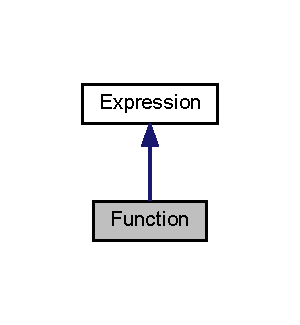
\includegraphics[width=144pt]{class_function__inherit__graph}
\end{center}
\end{figure}


Collaboration diagram for Function\-:\nopagebreak
\begin{figure}[H]
\begin{center}
\leavevmode
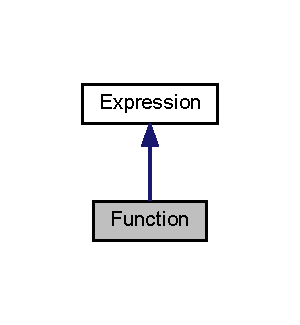
\includegraphics[width=144pt]{class_function__coll__graph}
\end{center}
\end{figure}
\subsection*{Public Member Functions}
\begin{DoxyCompactItemize}
\item 
\hyperlink{class_function_a508de932e951e7149bf67a71add8b767}{Function} (std\-::string body, std\-::string name)
\begin{DoxyCompactList}\small\item\em Constructor. \end{DoxyCompactList}\item 
\hypertarget{class_function_a3b03f7cf0b75d16edebdda1dee1db6fd}{virtual \hyperlink{class_function_a3b03f7cf0b75d16edebdda1dee1db6fd}{$\sim$\-Function} ()}\label{class_function_a3b03f7cf0b75d16edebdda1dee1db6fd}

\begin{DoxyCompactList}\small\item\em Destructor. \end{DoxyCompactList}\item 
std\-::string \hyperlink{class_function_a5b7d859d767e8a9c19fc5b81a0d10395}{get\-Name} ()
\begin{DoxyCompactList}\small\item\em Return the name of the function. \end{DoxyCompactList}\item 
void \hyperlink{class_function_a31a31e029daa1e11d0d58441bf5eb03f}{set\-Name} (std\-::string name)
\begin{DoxyCompactList}\small\item\em Modify the name of the function. \end{DoxyCompactList}\item 
void \hyperlink{class_function_a7ea0df19722e961d9001f7bfbae5262e}{set\-Args\-Names} (std\-::list$<$ std\-::string $>$ $\ast$args)
\begin{DoxyCompactList}\small\item\em Modify arguments of the function. \end{DoxyCompactList}\item 
\hyperlink{class_abstract_number}{Abstract\-Number} $\ast$ \hyperlink{class_function_af855f870a867e5fadaa23c4fb54bdc2d}{eval} (std\-::list$<$ \hyperlink{class_expression}{Expression} $\ast$ $>$ $\ast$args)
\begin{DoxyCompactList}\small\item\em Evaluate the function. \end{DoxyCompactList}\item 
\hyperlink{class_abstract_number}{Abstract\-Number} $\ast$ \hyperlink{class_function_afb64e5f34ae75847a68ab79c06a553cb}{eval} ()
\begin{DoxyCompactList}\small\item\em Evaluate the function's body. \end{DoxyCompactList}\item 
\hyperlink{class_number}{Number} $\ast$ \hyperlink{class_function_a1d0b8e117cd137e34ab843cc9e28ed53}{get\-Arg} (std\-::string name)
\begin{DoxyCompactList}\small\item\em Return the value associated with an argument in the local context. \end{DoxyCompactList}\item 
\hyperlink{class_expression}{Expression} $\ast$ \hyperlink{class_function_afaaf297558b5d18a51e04e9f5e20d270}{get\-Expression} ()
\begin{DoxyCompactList}\small\item\em Return the body expression. \end{DoxyCompactList}\item 
void \hyperlink{class_function_afcffaebf46fdb7f1ed0f689ae4078e45}{set\-Expression} (\hyperlink{class_expression}{Expression} $\ast$expr)
\begin{DoxyCompactList}\small\item\em Modify the body expression. \end{DoxyCompactList}\end{DoxyCompactItemize}
\subsection*{Additional Inherited Members}


\subsection{Detailed Description}
Represents an A\-S\-T function. 

\begin{DoxyAuthor}{Author}
David Lecoconnier 

Allan Mottier 
\end{DoxyAuthor}
\begin{DoxyDate}{Date}
2013-\/11-\/24 
\end{DoxyDate}


\subsection{Constructor \& Destructor Documentation}
\hypertarget{class_function_a508de932e951e7149bf67a71add8b767}{\index{Function@{Function}!Function@{Function}}
\index{Function@{Function}!Function@{Function}}
\subsubsection[{Function}]{\setlength{\rightskip}{0pt plus 5cm}Function\-::\-Function (
\begin{DoxyParamCaption}
\item[{std\-::string}]{body, }
\item[{std\-::string}]{name}
\end{DoxyParamCaption}
)}}\label{class_function_a508de932e951e7149bf67a71add8b767}


Constructor. 


\begin{DoxyParams}{Parameters}
{\em body} & text contained \\
\hline
{\em name} & the function name \\
\hline
\end{DoxyParams}


\subsection{Member Function Documentation}
\hypertarget{class_function_af855f870a867e5fadaa23c4fb54bdc2d}{\index{Function@{Function}!eval@{eval}}
\index{eval@{eval}!Function@{Function}}
\subsubsection[{eval}]{\setlength{\rightskip}{0pt plus 5cm}{\bf Abstract\-Number} $\ast$ Function\-::eval (
\begin{DoxyParamCaption}
\item[{std\-::list$<$ {\bf Expression} $\ast$ $>$ $\ast$}]{args}
\end{DoxyParamCaption}
)\hspace{0.3cm}{\ttfamily [virtual]}}}\label{class_function_af855f870a867e5fadaa23c4fb54bdc2d}


Evaluate the function. 


\begin{DoxyParams}{Parameters}
{\em args} & a list of arguments \\
\hline
\end{DoxyParams}
\begin{DoxyReturn}{Returns}
a \hyperlink{class_number}{Number} 
\end{DoxyReturn}


Implements \hyperlink{class_expression}{Expression}.

\hypertarget{class_function_afb64e5f34ae75847a68ab79c06a553cb}{\index{Function@{Function}!eval@{eval}}
\index{eval@{eval}!Function@{Function}}
\subsubsection[{eval}]{\setlength{\rightskip}{0pt plus 5cm}{\bf Abstract\-Number} $\ast$ Function\-::eval (
\begin{DoxyParamCaption}
{}
\end{DoxyParamCaption}
)}}\label{class_function_afb64e5f34ae75847a68ab79c06a553cb}


Evaluate the function's body. 

\begin{DoxyReturn}{Returns}
the evaluation's result 
\end{DoxyReturn}
\hypertarget{class_function_a1d0b8e117cd137e34ab843cc9e28ed53}{\index{Function@{Function}!get\-Arg@{get\-Arg}}
\index{get\-Arg@{get\-Arg}!Function@{Function}}
\subsubsection[{get\-Arg}]{\setlength{\rightskip}{0pt plus 5cm}{\bf Number} $\ast$ Function\-::get\-Arg (
\begin{DoxyParamCaption}
\item[{std\-::string}]{name}
\end{DoxyParamCaption}
)}}\label{class_function_a1d0b8e117cd137e34ab843cc9e28ed53}


Return the value associated with an argument in the local context. 


\begin{DoxyParams}{Parameters}
{\em name} & the name of the wanted argument \\
\hline
\end{DoxyParams}
\begin{DoxyReturn}{Returns}
a \hyperlink{class_number}{Number} 
\end{DoxyReturn}
\hypertarget{class_function_afaaf297558b5d18a51e04e9f5e20d270}{\index{Function@{Function}!get\-Expression@{get\-Expression}}
\index{get\-Expression@{get\-Expression}!Function@{Function}}
\subsubsection[{get\-Expression}]{\setlength{\rightskip}{0pt plus 5cm}{\bf Expression} $\ast$ Function\-::get\-Expression (
\begin{DoxyParamCaption}
{}
\end{DoxyParamCaption}
)}}\label{class_function_afaaf297558b5d18a51e04e9f5e20d270}


Return the body expression. 

\begin{DoxyReturn}{Returns}
the body 
\end{DoxyReturn}
\hypertarget{class_function_a5b7d859d767e8a9c19fc5b81a0d10395}{\index{Function@{Function}!get\-Name@{get\-Name}}
\index{get\-Name@{get\-Name}!Function@{Function}}
\subsubsection[{get\-Name}]{\setlength{\rightskip}{0pt plus 5cm}std\-::string Function\-::get\-Name (
\begin{DoxyParamCaption}
{}
\end{DoxyParamCaption}
)}}\label{class_function_a5b7d859d767e8a9c19fc5b81a0d10395}


Return the name of the function. 

\begin{DoxyReturn}{Returns}
the name 
\end{DoxyReturn}
\hypertarget{class_function_a7ea0df19722e961d9001f7bfbae5262e}{\index{Function@{Function}!set\-Args\-Names@{set\-Args\-Names}}
\index{set\-Args\-Names@{set\-Args\-Names}!Function@{Function}}
\subsubsection[{set\-Args\-Names}]{\setlength{\rightskip}{0pt plus 5cm}void Function\-::set\-Args\-Names (
\begin{DoxyParamCaption}
\item[{std\-::list$<$ std\-::string $>$ $\ast$}]{args}
\end{DoxyParamCaption}
)}}\label{class_function_a7ea0df19722e961d9001f7bfbae5262e}


Modify arguments of the function. 


\begin{DoxyParams}{Parameters}
{\em list} & a list of names \\
\hline
\end{DoxyParams}
\hypertarget{class_function_afcffaebf46fdb7f1ed0f689ae4078e45}{\index{Function@{Function}!set\-Expression@{set\-Expression}}
\index{set\-Expression@{set\-Expression}!Function@{Function}}
\subsubsection[{set\-Expression}]{\setlength{\rightskip}{0pt plus 5cm}void Function\-::set\-Expression (
\begin{DoxyParamCaption}
\item[{{\bf Expression} $\ast$}]{expr}
\end{DoxyParamCaption}
)}}\label{class_function_afcffaebf46fdb7f1ed0f689ae4078e45}


Modify the body expression. 


\begin{DoxyParams}{Parameters}
{\em expr} & an \hyperlink{class_expression}{Expression} \\
\hline
\end{DoxyParams}
\hypertarget{class_function_a31a31e029daa1e11d0d58441bf5eb03f}{\index{Function@{Function}!set\-Name@{set\-Name}}
\index{set\-Name@{set\-Name}!Function@{Function}}
\subsubsection[{set\-Name}]{\setlength{\rightskip}{0pt plus 5cm}void Function\-::set\-Name (
\begin{DoxyParamCaption}
\item[{std\-::string}]{name}
\end{DoxyParamCaption}
)}}\label{class_function_a31a31e029daa1e11d0d58441bf5eb03f}


Modify the name of the function. 


\begin{DoxyParams}{Parameters}
{\em name} & a new name \\
\hline
\end{DoxyParams}


The documentation for this class was generated from the following files\-:\begin{DoxyCompactItemize}
\item 
include/\-Functions/Function.\-h\item 
src/\-Functions/Function.\-cpp\end{DoxyCompactItemize}

\hypertarget{class_global_context}{\section{Global\-Context Class Reference}
\label{class_global_context}\index{Global\-Context@{Global\-Context}}
}


\hyperlink{class_context}{Context} which is always available. This context manages all locals contexts.  




Inheritance diagram for Global\-Context\-:\nopagebreak
\begin{figure}[H]
\begin{center}
\leavevmode
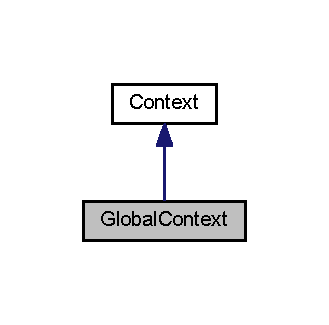
\includegraphics[width=158pt]{class_global_context__inherit__graph}
\end{center}
\end{figure}


Collaboration diagram for Global\-Context\-:\nopagebreak
\begin{figure}[H]
\begin{center}
\leavevmode
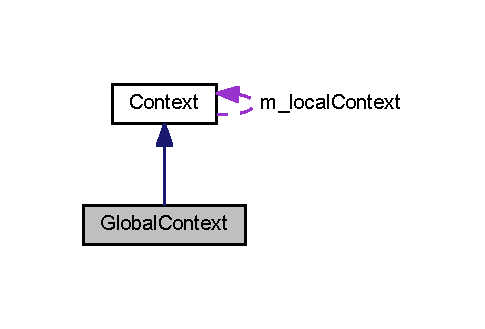
\includegraphics[width=233pt]{class_global_context__coll__graph}
\end{center}
\end{figure}
\subsection*{Static Public Member Functions}
\begin{DoxyCompactItemize}
\item 
\hypertarget{class_global_context_a1ccee0c92d355aa269004a7eac17c07f}{static \hyperlink{class_global_context}{Global\-Context} $\ast$ \hyperlink{class_global_context_a1ccee0c92d355aa269004a7eac17c07f}{get\-Instance} ()}\label{class_global_context_a1ccee0c92d355aa269004a7eac17c07f}

\begin{DoxyCompactList}\small\item\em Singleton. \end{DoxyCompactList}\end{DoxyCompactItemize}
\subsection*{Additional Inherited Members}


\subsection{Detailed Description}
\hyperlink{class_context}{Context} which is always available. This context manages all locals contexts. 

\begin{DoxyAuthor}{Author}
David Lecoconnier 

Allan Mottier 
\end{DoxyAuthor}
\begin{DoxyDate}{Date}
2013-\/11-\/24 
\end{DoxyDate}


The documentation for this class was generated from the following files\-:\begin{DoxyCompactItemize}
\item 
include/\-Memory/Global\-Context.\-h\item 
src/\-Memory/Global\-Context.\-cpp\end{DoxyCompactItemize}

\hypertarget{class_global_functions}{\section{Global\-Functions Class Reference}
\label{class_global_functions}\index{Global\-Functions@{Global\-Functions}}
}


Pool of all evaluated functions.  


\subsection*{Public Member Functions}
\begin{DoxyCompactItemize}
\item 
bool \hyperlink{class_global_functions_acef0e746c933a653d646c011386e2751}{is\-Containing} (std\-::string name)
\begin{DoxyCompactList}\small\item\em Test the presence of a function. \end{DoxyCompactList}\item 
\hyperlink{class_function}{Function} $\ast$ \hyperlink{class_global_functions_a22419333b2eadadb78d3e4022cc39fb2}{get\-Funtion} (std\-::string name)
\begin{DoxyCompactList}\small\item\em Return an evaluated function. \end{DoxyCompactList}\item 
void \hyperlink{class_global_functions_a9f41b87b5aae62b5e986a74f6bc34754}{add\-Function} (std\-::string name, \hyperlink{class_function}{Function} $\ast$funct)
\begin{DoxyCompactList}\small\item\em \hyperlink{class_add}{Add} a new function in the pool. \end{DoxyCompactList}\end{DoxyCompactItemize}
\subsection*{Static Public Member Functions}
\begin{DoxyCompactItemize}
\item 
\hypertarget{class_global_functions_a3ea0c14884cd6361b38755906113598b}{static \hyperlink{class_global_functions}{Global\-Functions} $\ast$ \hyperlink{class_global_functions_a3ea0c14884cd6361b38755906113598b}{get\-Instance} ()}\label{class_global_functions_a3ea0c14884cd6361b38755906113598b}

\begin{DoxyCompactList}\small\item\em Singleton. \end{DoxyCompactList}\end{DoxyCompactItemize}


\subsection{Detailed Description}
Pool of all evaluated functions. 

\begin{DoxyAuthor}{Author}
David Lecoconnier 

Allan Mottier 
\end{DoxyAuthor}
\begin{DoxyDate}{Date}
2013-\/11-\/24 
\end{DoxyDate}


\subsection{Member Function Documentation}
\hypertarget{class_global_functions_a9f41b87b5aae62b5e986a74f6bc34754}{\index{Global\-Functions@{Global\-Functions}!add\-Function@{add\-Function}}
\index{add\-Function@{add\-Function}!GlobalFunctions@{Global\-Functions}}
\subsubsection[{add\-Function}]{\setlength{\rightskip}{0pt plus 5cm}void Global\-Functions\-::add\-Function (
\begin{DoxyParamCaption}
\item[{std\-::string}]{name, }
\item[{{\bf Function} $\ast$}]{funct}
\end{DoxyParamCaption}
)}}\label{class_global_functions_a9f41b87b5aae62b5e986a74f6bc34754}


\hyperlink{class_add}{Add} a new function in the pool. 

If the function is already in the pool, the new definition replaces the old one. 
\begin{DoxyParams}{Parameters}
{\em name} & name of the function \\
\hline
{\em funct} & the function to add \\
\hline
\end{DoxyParams}
\hypertarget{class_global_functions_a22419333b2eadadb78d3e4022cc39fb2}{\index{Global\-Functions@{Global\-Functions}!get\-Funtion@{get\-Funtion}}
\index{get\-Funtion@{get\-Funtion}!GlobalFunctions@{Global\-Functions}}
\subsubsection[{get\-Funtion}]{\setlength{\rightskip}{0pt plus 5cm}{\bf Function} $\ast$ Global\-Functions\-::get\-Funtion (
\begin{DoxyParamCaption}
\item[{std\-::string}]{name}
\end{DoxyParamCaption}
)}}\label{class_global_functions_a22419333b2eadadb78d3e4022cc39fb2}


Return an evaluated function. 


\begin{DoxyParams}{Parameters}
{\em name} & name of the function \\
\hline
\end{DoxyParams}
\begin{DoxyReturn}{Returns}
the function name 
\end{DoxyReturn}
\hypertarget{class_global_functions_acef0e746c933a653d646c011386e2751}{\index{Global\-Functions@{Global\-Functions}!is\-Containing@{is\-Containing}}
\index{is\-Containing@{is\-Containing}!GlobalFunctions@{Global\-Functions}}
\subsubsection[{is\-Containing}]{\setlength{\rightskip}{0pt plus 5cm}bool Global\-Functions\-::is\-Containing (
\begin{DoxyParamCaption}
\item[{std\-::string}]{name}
\end{DoxyParamCaption}
)}}\label{class_global_functions_acef0e746c933a653d646c011386e2751}


Test the presence of a function. 


\begin{DoxyParams}{Parameters}
{\em name} & the name of a function \\
\hline
\end{DoxyParams}
\begin{DoxyReturn}{Returns}
true if present 
\end{DoxyReturn}


The documentation for this class was generated from the following files\-:\begin{DoxyCompactItemize}
\item 
include/\-Functions/Global\-Functions.\-h\item 
src/\-Functions/Global\-Functions.\-cpp\end{DoxyCompactItemize}

\hypertarget{class_if_then_else}{\section{If\-Then\-Else Class Reference}
\label{class_if_then_else}\index{If\-Then\-Else@{If\-Then\-Else}}
}


If expression.  




Inheritance diagram for If\-Then\-Else\-:\nopagebreak
\begin{figure}[H]
\begin{center}
\leavevmode
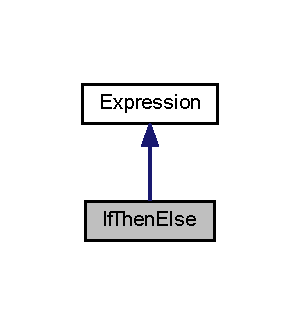
\includegraphics[width=144pt]{class_if_then_else__inherit__graph}
\end{center}
\end{figure}


Collaboration diagram for If\-Then\-Else\-:\nopagebreak
\begin{figure}[H]
\begin{center}
\leavevmode
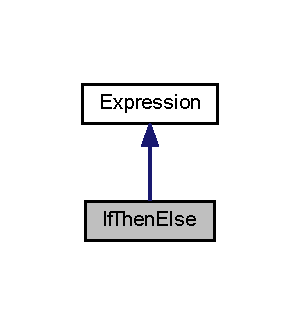
\includegraphics[width=144pt]{class_if_then_else__coll__graph}
\end{center}
\end{figure}
\subsection*{Public Member Functions}
\begin{DoxyCompactItemize}
\item 
\hyperlink{class_if_then_else_abf6f0e5ecce77a24b5cee1e31190818f}{If\-Then\-Else} (std\-::string body)
\begin{DoxyCompactList}\small\item\em Constructor. \end{DoxyCompactList}\item 
\hypertarget{class_if_then_else_a14d1c1cea52dd3b9939de1e6b54b86c6}{virtual \hyperlink{class_if_then_else_a14d1c1cea52dd3b9939de1e6b54b86c6}{$\sim$\-If\-Then\-Else} ()}\label{class_if_then_else_a14d1c1cea52dd3b9939de1e6b54b86c6}

\begin{DoxyCompactList}\small\item\em Destructor. \end{DoxyCompactList}\item 
virtual \hyperlink{class_abstract_number}{Abstract\-Number} $\ast$ \hyperlink{class_if_then_else_af535b187cfbd3a2f7ea3704d23dbcfa8}{eval} (std\-::list$<$ \hyperlink{class_expression}{Expression} $\ast$ $>$ $\ast$args)
\begin{DoxyCompactList}\small\item\em Evaluate the if. \end{DoxyCompactList}\item 
\-::\hyperlink{class_expression}{Expression} $\ast$ \hyperlink{class_if_then_else_a90885fff45494cab3c6c2461ebfa7277}{get\-Left} ()
\begin{DoxyCompactList}\small\item\em Return the left expression. \end{DoxyCompactList}\item 
\-::\hyperlink{class_expression}{Expression} $\ast$ \hyperlink{class_if_then_else_ab2ffd8ec427ba4fa86284d21f1fe7f87}{get\-Right} ()
\begin{DoxyCompactList}\small\item\em Return the right expression. \end{DoxyCompactList}\item 
\hyperlink{class_boolean_condition}{Boolean\-Condition} $\ast$ \hyperlink{class_if_then_else_adfd61f38868f9e63d7ab3f61023ca39a}{get\-Condition} ()
\begin{DoxyCompactList}\small\item\em Return the condition. \end{DoxyCompactList}\item 
void \hyperlink{class_if_then_else_a0477e20916d36241b92ac64d799ea2c1}{set\-Left} (\-::\hyperlink{class_expression}{Expression} $\ast$left)
\begin{DoxyCompactList}\small\item\em Modify the left expression. \end{DoxyCompactList}\item 
void \hyperlink{class_if_then_else_a169fc4074f3ab0eee0c4ef107de8b6a2}{set\-Right} (\-::\hyperlink{class_expression}{Expression} $\ast$right)
\begin{DoxyCompactList}\small\item\em Modify the right expression. \end{DoxyCompactList}\item 
void \hyperlink{class_if_then_else_a9fdafff73584bfffebf3cc798f20b6cd}{set\-Bool\-Condition} (\hyperlink{class_boolean_condition}{Boolean\-Condition} $\ast$condition)
\begin{DoxyCompactList}\small\item\em Modify the boolean condition. \end{DoxyCompactList}\end{DoxyCompactItemize}
\subsection*{Additional Inherited Members}


\subsection{Detailed Description}
If expression. 

\begin{DoxyAuthor}{Author}
David Lecoconnier 

Allan Mottier 
\end{DoxyAuthor}
\begin{DoxyDate}{Date}
2013-\/11-\/24 
\end{DoxyDate}


\subsection{Constructor \& Destructor Documentation}
\hypertarget{class_if_then_else_abf6f0e5ecce77a24b5cee1e31190818f}{\index{If\-Then\-Else@{If\-Then\-Else}!If\-Then\-Else@{If\-Then\-Else}}
\index{If\-Then\-Else@{If\-Then\-Else}!IfThenElse@{If\-Then\-Else}}
\subsubsection[{If\-Then\-Else}]{\setlength{\rightskip}{0pt plus 5cm}If\-Then\-Else\-::\-If\-Then\-Else (
\begin{DoxyParamCaption}
\item[{std\-::string}]{body}
\end{DoxyParamCaption}
)}}\label{class_if_then_else_abf6f0e5ecce77a24b5cee1e31190818f}


Constructor. 


\begin{DoxyParams}{Parameters}
{\em body} & text contained \\
\hline
\end{DoxyParams}


\subsection{Member Function Documentation}
\hypertarget{class_if_then_else_af535b187cfbd3a2f7ea3704d23dbcfa8}{\index{If\-Then\-Else@{If\-Then\-Else}!eval@{eval}}
\index{eval@{eval}!IfThenElse@{If\-Then\-Else}}
\subsubsection[{eval}]{\setlength{\rightskip}{0pt plus 5cm}{\bf Abstract\-Number} $\ast$ If\-Then\-Else\-::eval (
\begin{DoxyParamCaption}
\item[{std\-::list$<$ {\bf Expression} $\ast$ $>$ $\ast$}]{args}
\end{DoxyParamCaption}
)\hspace{0.3cm}{\ttfamily [virtual]}}}\label{class_if_then_else_af535b187cfbd3a2f7ea3704d23dbcfa8}


Evaluate the if. 


\begin{DoxyParams}{Parameters}
{\em args} & a list of arguments -\/ Useless here \\
\hline
\end{DoxyParams}
\begin{DoxyReturn}{Returns}
the result of the evaluation 
\end{DoxyReturn}


Implements \hyperlink{class_expression}{Expression}.

\hypertarget{class_if_then_else_adfd61f38868f9e63d7ab3f61023ca39a}{\index{If\-Then\-Else@{If\-Then\-Else}!get\-Condition@{get\-Condition}}
\index{get\-Condition@{get\-Condition}!IfThenElse@{If\-Then\-Else}}
\subsubsection[{get\-Condition}]{\setlength{\rightskip}{0pt plus 5cm}{\bf Boolean\-Condition} $\ast$ If\-Then\-Else\-::get\-Condition (
\begin{DoxyParamCaption}
{}
\end{DoxyParamCaption}
)}}\label{class_if_then_else_adfd61f38868f9e63d7ab3f61023ca39a}


Return the condition. 

\begin{DoxyReturn}{Returns}
a boolean condition 
\end{DoxyReturn}
\hypertarget{class_if_then_else_a90885fff45494cab3c6c2461ebfa7277}{\index{If\-Then\-Else@{If\-Then\-Else}!get\-Left@{get\-Left}}
\index{get\-Left@{get\-Left}!IfThenElse@{If\-Then\-Else}}
\subsubsection[{get\-Left}]{\setlength{\rightskip}{0pt plus 5cm}{\bf Expression} $\ast$ If\-Then\-Else\-::get\-Left (
\begin{DoxyParamCaption}
{}
\end{DoxyParamCaption}
)}}\label{class_if_then_else_a90885fff45494cab3c6c2461ebfa7277}


Return the left expression. 

\begin{DoxyReturn}{Returns}
left part 
\end{DoxyReturn}
\hypertarget{class_if_then_else_ab2ffd8ec427ba4fa86284d21f1fe7f87}{\index{If\-Then\-Else@{If\-Then\-Else}!get\-Right@{get\-Right}}
\index{get\-Right@{get\-Right}!IfThenElse@{If\-Then\-Else}}
\subsubsection[{get\-Right}]{\setlength{\rightskip}{0pt plus 5cm}{\bf Expression} $\ast$ If\-Then\-Else\-::get\-Right (
\begin{DoxyParamCaption}
{}
\end{DoxyParamCaption}
)}}\label{class_if_then_else_ab2ffd8ec427ba4fa86284d21f1fe7f87}


Return the right expression. 

\begin{DoxyReturn}{Returns}
right part 
\end{DoxyReturn}
\hypertarget{class_if_then_else_a9fdafff73584bfffebf3cc798f20b6cd}{\index{If\-Then\-Else@{If\-Then\-Else}!set\-Bool\-Condition@{set\-Bool\-Condition}}
\index{set\-Bool\-Condition@{set\-Bool\-Condition}!IfThenElse@{If\-Then\-Else}}
\subsubsection[{set\-Bool\-Condition}]{\setlength{\rightskip}{0pt plus 5cm}void If\-Then\-Else\-::set\-Bool\-Condition (
\begin{DoxyParamCaption}
\item[{{\bf Boolean\-Condition} $\ast$}]{condition}
\end{DoxyParamCaption}
)}}\label{class_if_then_else_a9fdafff73584bfffebf3cc798f20b6cd}


Modify the boolean condition. 


\begin{DoxyParams}{Parameters}
{\em condition} & a boolean condition \\
\hline
\end{DoxyParams}
\hypertarget{class_if_then_else_a0477e20916d36241b92ac64d799ea2c1}{\index{If\-Then\-Else@{If\-Then\-Else}!set\-Left@{set\-Left}}
\index{set\-Left@{set\-Left}!IfThenElse@{If\-Then\-Else}}
\subsubsection[{set\-Left}]{\setlength{\rightskip}{0pt plus 5cm}void If\-Then\-Else\-::set\-Left (
\begin{DoxyParamCaption}
\item[{\-::{\bf Expression} $\ast$}]{left}
\end{DoxyParamCaption}
)}}\label{class_if_then_else_a0477e20916d36241b92ac64d799ea2c1}


Modify the left expression. 


\begin{DoxyParams}{Parameters}
{\em left} & left part \\
\hline
\end{DoxyParams}
\hypertarget{class_if_then_else_a169fc4074f3ab0eee0c4ef107de8b6a2}{\index{If\-Then\-Else@{If\-Then\-Else}!set\-Right@{set\-Right}}
\index{set\-Right@{set\-Right}!IfThenElse@{If\-Then\-Else}}
\subsubsection[{set\-Right}]{\setlength{\rightskip}{0pt plus 5cm}void If\-Then\-Else\-::set\-Right (
\begin{DoxyParamCaption}
\item[{\-::{\bf Expression} $\ast$}]{right}
\end{DoxyParamCaption}
)}}\label{class_if_then_else_a169fc4074f3ab0eee0c4ef107de8b6a2}


Modify the right expression. 


\begin{DoxyParams}{Parameters}
{\em right} & right part \\
\hline
\end{DoxyParams}


The documentation for this class was generated from the following files\-:\begin{DoxyCompactItemize}
\item 
include/\-Functions/If\-Then\-Else.\-h\item 
src/\-Functions/If\-Then\-Else.\-cpp\end{DoxyCompactItemize}

\hypertarget{class_less_than_or_equal}{\section{Less\-Than\-Or\-Equal Class Reference}
\label{class_less_than_or_equal}\index{Less\-Than\-Or\-Equal@{Less\-Than\-Or\-Equal}}
}


A\-S\-T '$<$=' boolean expression.  




Inheritance diagram for Less\-Than\-Or\-Equal\-:\nopagebreak
\begin{figure}[H]
\begin{center}
\leavevmode
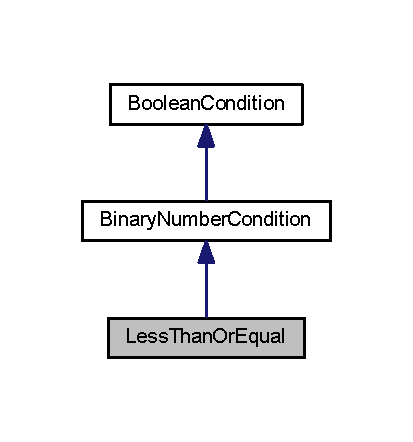
\includegraphics[width=198pt]{class_less_than_or_equal__inherit__graph}
\end{center}
\end{figure}


Collaboration diagram for Less\-Than\-Or\-Equal\-:\nopagebreak
\begin{figure}[H]
\begin{center}
\leavevmode
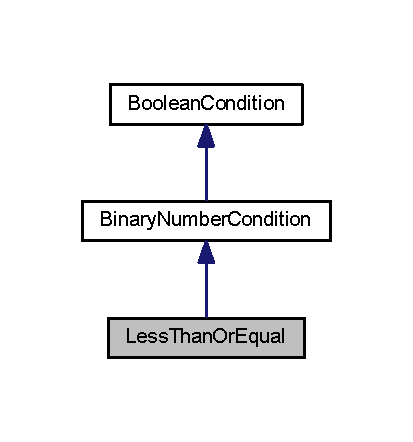
\includegraphics[width=198pt]{class_less_than_or_equal__coll__graph}
\end{center}
\end{figure}
\subsection*{Public Member Functions}
\begin{DoxyCompactItemize}
\item 
\hyperlink{class_less_than_or_equal_a2426e20f4e879e169e4554cd152ab4ae}{Less\-Than\-Or\-Equal} (std\-::string body)
\begin{DoxyCompactList}\small\item\em Constructor. \end{DoxyCompactList}\item 
\hypertarget{class_less_than_or_equal_ac7ff9a98ce2b5c5f83ba25f9b992f4b8}{virtual \hyperlink{class_less_than_or_equal_ac7ff9a98ce2b5c5f83ba25f9b992f4b8}{$\sim$\-Less\-Than\-Or\-Equal} ()}\label{class_less_than_or_equal_ac7ff9a98ce2b5c5f83ba25f9b992f4b8}

\begin{DoxyCompactList}\small\item\em Destructor. \end{DoxyCompactList}\item 
bool \hyperlink{class_less_than_or_equal_a54995a50037c8931b76767e64d038f3a}{eval} ()
\begin{DoxyCompactList}\small\item\em Evaluate the difference between left member and right member. \end{DoxyCompactList}\end{DoxyCompactItemize}
\subsection*{Additional Inherited Members}


\subsection{Detailed Description}
A\-S\-T '$<$=' boolean expression. 

\begin{DoxyAuthor}{Author}
David Lecoconnier 

Allan Mottier 
\end{DoxyAuthor}
\begin{DoxyDate}{Date}
2013-\/11-\/24 
\end{DoxyDate}


\subsection{Constructor \& Destructor Documentation}
\hypertarget{class_less_than_or_equal_a2426e20f4e879e169e4554cd152ab4ae}{\index{Less\-Than\-Or\-Equal@{Less\-Than\-Or\-Equal}!Less\-Than\-Or\-Equal@{Less\-Than\-Or\-Equal}}
\index{Less\-Than\-Or\-Equal@{Less\-Than\-Or\-Equal}!LessThanOrEqual@{Less\-Than\-Or\-Equal}}
\subsubsection[{Less\-Than\-Or\-Equal}]{\setlength{\rightskip}{0pt plus 5cm}Less\-Than\-Or\-Equal\-::\-Less\-Than\-Or\-Equal (
\begin{DoxyParamCaption}
\item[{std\-::string}]{body}
\end{DoxyParamCaption}
)}}\label{class_less_than_or_equal_a2426e20f4e879e169e4554cd152ab4ae}


Constructor. 


\begin{DoxyParams}{Parameters}
{\em body} & text \\
\hline
\end{DoxyParams}


\subsection{Member Function Documentation}
\hypertarget{class_less_than_or_equal_a54995a50037c8931b76767e64d038f3a}{\index{Less\-Than\-Or\-Equal@{Less\-Than\-Or\-Equal}!eval@{eval}}
\index{eval@{eval}!LessThanOrEqual@{Less\-Than\-Or\-Equal}}
\subsubsection[{eval}]{\setlength{\rightskip}{0pt plus 5cm}bool Less\-Than\-Or\-Equal\-::eval (
\begin{DoxyParamCaption}
{}
\end{DoxyParamCaption}
)\hspace{0.3cm}{\ttfamily [virtual]}}}\label{class_less_than_or_equal_a54995a50037c8931b76767e64d038f3a}


Evaluate the difference between left member and right member. 

\begin{DoxyReturn}{Returns}
return true if left $<$= right 
\end{DoxyReturn}


Implements \hyperlink{class_boolean_condition}{Boolean\-Condition}.



The documentation for this class was generated from the following files\-:\begin{DoxyCompactItemize}
\item 
include/\-Booleans/Less\-Than\-Or\-Equal.\-h\item 
src/\-Booleans/Less\-Than\-Or\-Equal.\-cpp\end{DoxyCompactItemize}

\hypertarget{class_modulo}{\section{Modulo Class Reference}
\label{class_modulo}\index{Modulo@{Modulo}}
}


\hyperlink{class_modulo}{Modulo} operation.  




Inheritance diagram for Modulo\-:\nopagebreak
\begin{figure}[H]
\begin{center}
\leavevmode
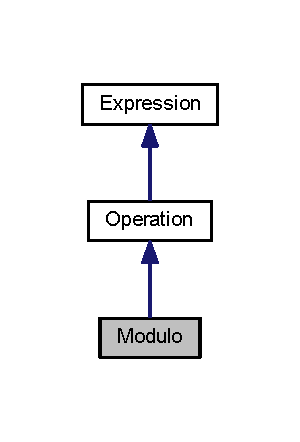
\includegraphics[width=144pt]{class_modulo__inherit__graph}
\end{center}
\end{figure}


Collaboration diagram for Modulo\-:\nopagebreak
\begin{figure}[H]
\begin{center}
\leavevmode
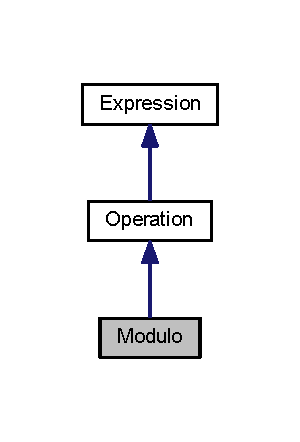
\includegraphics[width=144pt]{class_modulo__coll__graph}
\end{center}
\end{figure}
\subsection*{Public Member Functions}
\begin{DoxyCompactItemize}
\item 
\hyperlink{class_modulo_abecede722d0e86774c16a8a81d0b44d0}{Modulo} (std\-::string body)
\begin{DoxyCompactList}\small\item\em Default constructor. \end{DoxyCompactList}\item 
virtual \hyperlink{class_modulo_a8461196a9b9a9dbe2ee75a7f263d49e2}{$\sim$\-Modulo} ()
\begin{DoxyCompactList}\small\item\em Default destructor. \end{DoxyCompactList}\item 
virtual \hyperlink{class_abstract_number}{Abstract\-Number} $\ast$ \hyperlink{class_modulo_acc08e59b645a37ebfe94f03d490a627c}{eval} (std\-::list$<$ \hyperlink{class_expression}{Expression} $\ast$ $>$ $\ast$args)
\begin{DoxyCompactList}\small\item\em Evaluate the \hyperlink{class_modulo}{Modulo} operation. \end{DoxyCompactList}\end{DoxyCompactItemize}
\subsection*{Additional Inherited Members}


\subsection{Detailed Description}
\hyperlink{class_modulo}{Modulo} operation. 

\begin{DoxyAuthor}{Author}
David Lecoconnier 

Allan Mottier 
\end{DoxyAuthor}
\begin{DoxyDate}{Date}
2013-\/11-\/24 
\end{DoxyDate}


\subsection{Constructor \& Destructor Documentation}
\hypertarget{class_modulo_abecede722d0e86774c16a8a81d0b44d0}{\index{Modulo@{Modulo}!Modulo@{Modulo}}
\index{Modulo@{Modulo}!Modulo@{Modulo}}
\subsubsection[{Modulo}]{\setlength{\rightskip}{0pt plus 5cm}Modulo\-::\-Modulo (
\begin{DoxyParamCaption}
\item[{std\-::string}]{body}
\end{DoxyParamCaption}
)}}\label{class_modulo_abecede722d0e86774c16a8a81d0b44d0}


Default constructor. 

Constructor.


\begin{DoxyParams}{Parameters}
{\em body} & text contained \\
\hline
\end{DoxyParams}
\hypertarget{class_modulo_a8461196a9b9a9dbe2ee75a7f263d49e2}{\index{Modulo@{Modulo}!$\sim$\-Modulo@{$\sim$\-Modulo}}
\index{$\sim$\-Modulo@{$\sim$\-Modulo}!Modulo@{Modulo}}
\subsubsection[{$\sim$\-Modulo}]{\setlength{\rightskip}{0pt plus 5cm}Modulo\-::$\sim$\-Modulo (
\begin{DoxyParamCaption}
{}
\end{DoxyParamCaption}
)\hspace{0.3cm}{\ttfamily [virtual]}}}\label{class_modulo_a8461196a9b9a9dbe2ee75a7f263d49e2}


Default destructor. 

Destructor. 

\subsection{Member Function Documentation}
\hypertarget{class_modulo_acc08e59b645a37ebfe94f03d490a627c}{\index{Modulo@{Modulo}!eval@{eval}}
\index{eval@{eval}!Modulo@{Modulo}}
\subsubsection[{eval}]{\setlength{\rightskip}{0pt plus 5cm}{\bf Abstract\-Number} $\ast$ Modulo\-::eval (
\begin{DoxyParamCaption}
\item[{std\-::list$<$ {\bf Expression} $\ast$ $>$ $\ast$}]{args}
\end{DoxyParamCaption}
)\hspace{0.3cm}{\ttfamily [virtual]}}}\label{class_modulo_acc08e59b645a37ebfe94f03d490a627c}


Evaluate the \hyperlink{class_modulo}{Modulo} operation. 


\begin{DoxyParams}{Parameters}
{\em args} & -\/\-Useless-\/ \\
\hline
\end{DoxyParams}
\begin{DoxyReturn}{Returns}
the result 
\end{DoxyReturn}


Implements \hyperlink{class_expression}{Expression}.



The documentation for this class was generated from the following files\-:\begin{DoxyCompactItemize}
\item 
include/\-Numbers/Modulo.\-h\item 
src/\-Numbers/Modulo.\-cpp\end{DoxyCompactItemize}

\hypertarget{class_n_o_t}{\section{N\-O\-T Class Reference}
\label{class_n_o_t}\index{N\-O\-T@{N\-O\-T}}
}


\hyperlink{class_n_o_t}{N\-O\-T} operator.  




Inheritance diagram for N\-O\-T\-:\nopagebreak
\begin{figure}[H]
\begin{center}
\leavevmode
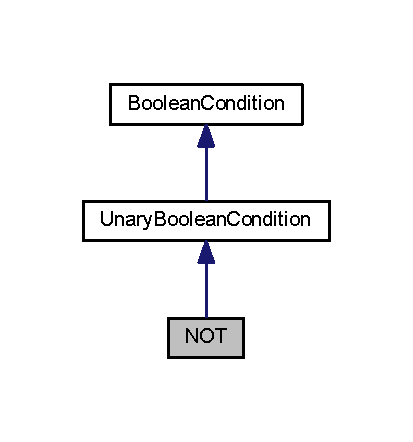
\includegraphics[width=198pt]{class_n_o_t__inherit__graph}
\end{center}
\end{figure}


Collaboration diagram for N\-O\-T\-:\nopagebreak
\begin{figure}[H]
\begin{center}
\leavevmode
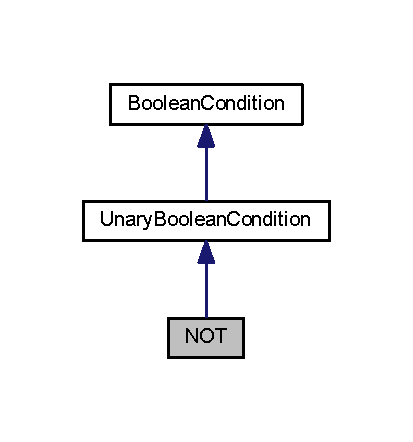
\includegraphics[width=198pt]{class_n_o_t__coll__graph}
\end{center}
\end{figure}
\subsection*{Public Member Functions}
\begin{DoxyCompactItemize}
\item 
\hyperlink{class_n_o_t_a1c7e836da1f35625dc95ada0de5ee76d}{N\-O\-T} (std\-::string body)
\begin{DoxyCompactList}\small\item\em Constructor. \end{DoxyCompactList}\item 
\hypertarget{class_n_o_t_ae73fa23af17cb3edb75f19aba9e364b0}{virtual \hyperlink{class_n_o_t_ae73fa23af17cb3edb75f19aba9e364b0}{$\sim$\-N\-O\-T} ()}\label{class_n_o_t_ae73fa23af17cb3edb75f19aba9e364b0}

\begin{DoxyCompactList}\small\item\em Destructor. \end{DoxyCompactList}\item 
virtual bool \hyperlink{class_n_o_t_a4606e14dae1f45f7fcaea60373d030db}{eval} ()
\begin{DoxyCompactList}\small\item\em Evaluate the not operator. \end{DoxyCompactList}\end{DoxyCompactItemize}
\subsection*{Additional Inherited Members}


\subsection{Detailed Description}
\hyperlink{class_n_o_t}{N\-O\-T} operator. 

\begin{DoxyAuthor}{Author}
David Lecoconnier 

Allan Mottier 
\end{DoxyAuthor}
\begin{DoxyDate}{Date}
2013-\/11-\/24 
\end{DoxyDate}


\subsection{Constructor \& Destructor Documentation}
\hypertarget{class_n_o_t_a1c7e836da1f35625dc95ada0de5ee76d}{\index{N\-O\-T@{N\-O\-T}!N\-O\-T@{N\-O\-T}}
\index{N\-O\-T@{N\-O\-T}!NOT@{N\-O\-T}}
\subsubsection[{N\-O\-T}]{\setlength{\rightskip}{0pt plus 5cm}N\-O\-T\-::\-N\-O\-T (
\begin{DoxyParamCaption}
\item[{std\-::string}]{body}
\end{DoxyParamCaption}
)}}\label{class_n_o_t_a1c7e836da1f35625dc95ada0de5ee76d}


Constructor. 


\begin{DoxyParams}{Parameters}
{\em body} & text contained \\
\hline
\end{DoxyParams}


\subsection{Member Function Documentation}
\hypertarget{class_n_o_t_a4606e14dae1f45f7fcaea60373d030db}{\index{N\-O\-T@{N\-O\-T}!eval@{eval}}
\index{eval@{eval}!NOT@{N\-O\-T}}
\subsubsection[{eval}]{\setlength{\rightskip}{0pt plus 5cm}bool N\-O\-T\-::eval (
\begin{DoxyParamCaption}
{}
\end{DoxyParamCaption}
)\hspace{0.3cm}{\ttfamily [virtual]}}}\label{class_n_o_t_a4606e14dae1f45f7fcaea60373d030db}


Evaluate the not operator. 

It returns the opposite value \begin{DoxyReturn}{Returns}
true if it is false 
\end{DoxyReturn}


Implements \hyperlink{class_boolean_condition}{Boolean\-Condition}.



The documentation for this class was generated from the following files\-:\begin{DoxyCompactItemize}
\item 
include/\-Booleans/N\-O\-T.\-h\item 
src/\-Booleans/N\-O\-T.\-cpp\end{DoxyCompactItemize}

\hypertarget{class_number}{\section{Number Class Reference}
\label{class_number}\index{Number@{Number}}
}


A number is a representation of real world. From outside, there is no difference between integers and floats.  




Inheritance diagram for Number\-:\nopagebreak
\begin{figure}[H]
\begin{center}
\leavevmode
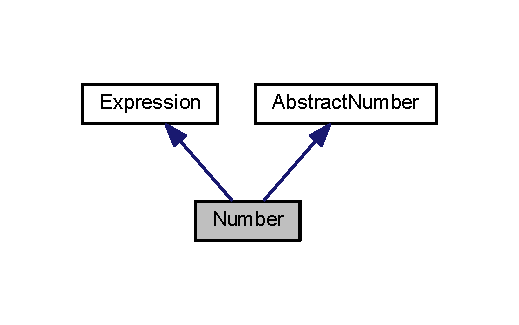
\includegraphics[width=249pt]{class_number__inherit__graph}
\end{center}
\end{figure}


Collaboration diagram for Number\-:\nopagebreak
\begin{figure}[H]
\begin{center}
\leavevmode
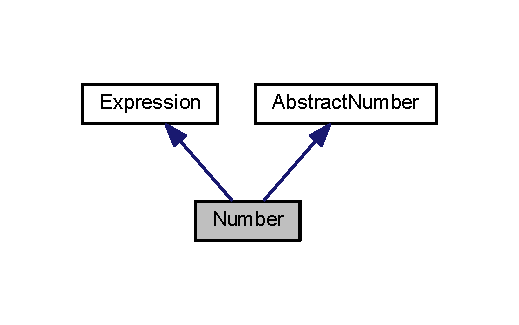
\includegraphics[width=249pt]{class_number__coll__graph}
\end{center}
\end{figure}
\subsection*{Public Member Functions}
\begin{DoxyCompactItemize}
\item 
\hyperlink{class_number_a055514cb4cb2727470a83e0df0905489}{Number} (int num)
\begin{DoxyCompactList}\small\item\em Default constructor. \end{DoxyCompactList}\item 
\hyperlink{class_number_a31ddc8a10dbfb7e2267d3e4d7a3b68f3}{Number} (float num)
\begin{DoxyCompactList}\small\item\em Constructor. \end{DoxyCompactList}\item 
\hyperlink{class_number_a2e57aec82986ef3b6700a8a22d4e5163}{Number} (std\-::string num)
\begin{DoxyCompactList}\small\item\em Constructor. \end{DoxyCompactList}\item 
virtual \hyperlink{class_number_a455be1ad651c9a6857276e992f31144c}{$\sim$\-Number} ()
\begin{DoxyCompactList}\small\item\em Default destructor. \end{DoxyCompactList}\item 
void \hyperlink{class_number_a9ddfb581d1ba880bec1f872987a5b031}{set\-Integer} (int val)
\begin{DoxyCompactList}\small\item\em Modify the value under integer form. \end{DoxyCompactList}\item 
void \hyperlink{class_number_a7a685cb10b55b64410086b374e0b5d97}{set\-Real} (double val)
\begin{DoxyCompactList}\small\item\em Modify the value under real form. \end{DoxyCompactList}\item 
bool \hyperlink{class_number_aa506c48f1ed35ea47807a29c8800510c}{is\-Real} ()
\begin{DoxyCompactList}\small\item\em Test number set. \end{DoxyCompactList}\item 
int \hyperlink{class_number_aef8e2baf2618ca24c077b7c285404629}{get\-Integer} ()
\begin{DoxyCompactList}\small\item\em Return the integer value. \end{DoxyCompactList}\item 
double \hyperlink{class_number_ab6e8e40c3104739f8cef48deb0dc048a}{get\-Real} ()
\begin{DoxyCompactList}\small\item\em Return the float value. \end{DoxyCompactList}\item 
std\-::string \hyperlink{class_number_a6fccb9ac17ca1aa8f3eec1ed10315348}{to\-String} ()
\begin{DoxyCompactList}\small\item\em Return the number under text form. \end{DoxyCompactList}\item 
void \hyperlink{class_number_abfd4a9fecbc0e56985893037cd066404}{from\-String} (std\-::string num)
\begin{DoxyCompactList}\small\item\em Modify the value. \end{DoxyCompactList}\item 
virtual \hyperlink{class_number}{Number} $\ast$ \hyperlink{class_number_af3b04493ef934bb571ebb71b8a5b4283}{eval} (std\-::list$<$ \hyperlink{class_expression}{Expression} $\ast$ $>$ $\ast$args)
\begin{DoxyCompactList}\small\item\em Evaluate the number. \end{DoxyCompactList}\item 
virtual \hyperlink{class_number}{Number} $\ast$ \hyperlink{class_number_ac6a27d78d44abe16f38d64f70cacf246}{eval} ()
\begin{DoxyCompactList}\small\item\em Evaluate the number. \end{DoxyCompactList}\end{DoxyCompactItemize}
\subsection*{Additional Inherited Members}


\subsection{Detailed Description}
A number is a representation of real world. From outside, there is no difference between integers and floats. 

\begin{DoxyAuthor}{Author}
David Lecoconnier 

Allan Mottier 
\end{DoxyAuthor}
\begin{DoxyDate}{Date}
2013-\/11-\/24 
\end{DoxyDate}


\subsection{Constructor \& Destructor Documentation}
\hypertarget{class_number_a055514cb4cb2727470a83e0df0905489}{\index{Number@{Number}!Number@{Number}}
\index{Number@{Number}!Number@{Number}}
\subsubsection[{Number}]{\setlength{\rightskip}{0pt plus 5cm}Number\-::\-Number (
\begin{DoxyParamCaption}
\item[{int}]{num}
\end{DoxyParamCaption}
)}}\label{class_number_a055514cb4cb2727470a83e0df0905489}


Default constructor. 

Constructor.


\begin{DoxyParams}{Parameters}
{\em num} & integer value \\
\hline
\end{DoxyParams}
\hypertarget{class_number_a31ddc8a10dbfb7e2267d3e4d7a3b68f3}{\index{Number@{Number}!Number@{Number}}
\index{Number@{Number}!Number@{Number}}
\subsubsection[{Number}]{\setlength{\rightskip}{0pt plus 5cm}Number\-::\-Number (
\begin{DoxyParamCaption}
\item[{float}]{num}
\end{DoxyParamCaption}
)}}\label{class_number_a31ddc8a10dbfb7e2267d3e4d7a3b68f3}


Constructor. 


\begin{DoxyParams}{Parameters}
{\em num} & real value \\
\hline
\end{DoxyParams}
\hypertarget{class_number_a2e57aec82986ef3b6700a8a22d4e5163}{\index{Number@{Number}!Number@{Number}}
\index{Number@{Number}!Number@{Number}}
\subsubsection[{Number}]{\setlength{\rightskip}{0pt plus 5cm}Number\-::\-Number (
\begin{DoxyParamCaption}
\item[{std\-::string}]{num}
\end{DoxyParamCaption}
)}}\label{class_number_a2e57aec82986ef3b6700a8a22d4e5163}


Constructor. 


\begin{DoxyParams}{Parameters}
{\em num} & value under text form \\
\hline
\end{DoxyParams}
\hypertarget{class_number_a455be1ad651c9a6857276e992f31144c}{\index{Number@{Number}!$\sim$\-Number@{$\sim$\-Number}}
\index{$\sim$\-Number@{$\sim$\-Number}!Number@{Number}}
\subsubsection[{$\sim$\-Number}]{\setlength{\rightskip}{0pt plus 5cm}Number\-::$\sim$\-Number (
\begin{DoxyParamCaption}
{}
\end{DoxyParamCaption}
)\hspace{0.3cm}{\ttfamily [virtual]}}}\label{class_number_a455be1ad651c9a6857276e992f31144c}


Default destructor. 

Destructor. 

\subsection{Member Function Documentation}
\hypertarget{class_number_af3b04493ef934bb571ebb71b8a5b4283}{\index{Number@{Number}!eval@{eval}}
\index{eval@{eval}!Number@{Number}}
\subsubsection[{eval}]{\setlength{\rightskip}{0pt plus 5cm}{\bf Number} $\ast$ Number\-::eval (
\begin{DoxyParamCaption}
\item[{std\-::list$<$ {\bf Expression} $\ast$ $>$ $\ast$}]{args}
\end{DoxyParamCaption}
)\hspace{0.3cm}{\ttfamily [virtual]}}}\label{class_number_af3b04493ef934bb571ebb71b8a5b4283}


Evaluate the number. 


\begin{DoxyParams}{Parameters}
{\em args} & -\/\-Useless-\/ \\
\hline
\end{DoxyParams}
\begin{DoxyReturn}{Returns}
this number 
\end{DoxyReturn}


Implements \hyperlink{class_expression}{Expression}.

\hypertarget{class_number_ac6a27d78d44abe16f38d64f70cacf246}{\index{Number@{Number}!eval@{eval}}
\index{eval@{eval}!Number@{Number}}
\subsubsection[{eval}]{\setlength{\rightskip}{0pt plus 5cm}{\bf Number} $\ast$ Number\-::eval (
\begin{DoxyParamCaption}
{}
\end{DoxyParamCaption}
)\hspace{0.3cm}{\ttfamily [virtual]}}}\label{class_number_ac6a27d78d44abe16f38d64f70cacf246}


Evaluate the number. 

\begin{DoxyReturn}{Returns}
this number 
\end{DoxyReturn}


Implements \hyperlink{class_abstract_number}{Abstract\-Number}.

\hypertarget{class_number_abfd4a9fecbc0e56985893037cd066404}{\index{Number@{Number}!from\-String@{from\-String}}
\index{from\-String@{from\-String}!Number@{Number}}
\subsubsection[{from\-String}]{\setlength{\rightskip}{0pt plus 5cm}void Number\-::from\-String (
\begin{DoxyParamCaption}
\item[{std\-::string}]{num}
\end{DoxyParamCaption}
)\hspace{0.3cm}{\ttfamily [virtual]}}}\label{class_number_abfd4a9fecbc0e56985893037cd066404}


Modify the value. 


\begin{DoxyParams}{Parameters}
{\em num} & a number under text form \\
\hline
\end{DoxyParams}


Implements \hyperlink{class_abstract_number}{Abstract\-Number}.

\hypertarget{class_number_aef8e2baf2618ca24c077b7c285404629}{\index{Number@{Number}!get\-Integer@{get\-Integer}}
\index{get\-Integer@{get\-Integer}!Number@{Number}}
\subsubsection[{get\-Integer}]{\setlength{\rightskip}{0pt plus 5cm}int Number\-::get\-Integer (
\begin{DoxyParamCaption}
{}
\end{DoxyParamCaption}
)\hspace{0.3cm}{\ttfamily [virtual]}}}\label{class_number_aef8e2baf2618ca24c077b7c285404629}


Return the integer value. 

\begin{DoxyReturn}{Returns}
an integer 
\end{DoxyReturn}


Implements \hyperlink{class_abstract_number}{Abstract\-Number}.

\hypertarget{class_number_ab6e8e40c3104739f8cef48deb0dc048a}{\index{Number@{Number}!get\-Real@{get\-Real}}
\index{get\-Real@{get\-Real}!Number@{Number}}
\subsubsection[{get\-Real}]{\setlength{\rightskip}{0pt plus 5cm}double Number\-::get\-Real (
\begin{DoxyParamCaption}
{}
\end{DoxyParamCaption}
)\hspace{0.3cm}{\ttfamily [virtual]}}}\label{class_number_ab6e8e40c3104739f8cef48deb0dc048a}


Return the float value. 

\begin{DoxyReturn}{Returns}
a float 
\end{DoxyReturn}


Implements \hyperlink{class_abstract_number}{Abstract\-Number}.

\hypertarget{class_number_aa506c48f1ed35ea47807a29c8800510c}{\index{Number@{Number}!is\-Real@{is\-Real}}
\index{is\-Real@{is\-Real}!Number@{Number}}
\subsubsection[{is\-Real}]{\setlength{\rightskip}{0pt plus 5cm}bool Number\-::is\-Real (
\begin{DoxyParamCaption}
{}
\end{DoxyParamCaption}
)\hspace{0.3cm}{\ttfamily [virtual]}}}\label{class_number_aa506c48f1ed35ea47807a29c8800510c}


Test number set. 

\begin{DoxyReturn}{Returns}
true if the number is in R 
\end{DoxyReturn}


Implements \hyperlink{class_abstract_number}{Abstract\-Number}.

\hypertarget{class_number_a9ddfb581d1ba880bec1f872987a5b031}{\index{Number@{Number}!set\-Integer@{set\-Integer}}
\index{set\-Integer@{set\-Integer}!Number@{Number}}
\subsubsection[{set\-Integer}]{\setlength{\rightskip}{0pt plus 5cm}void Number\-::set\-Integer (
\begin{DoxyParamCaption}
\item[{int}]{val}
\end{DoxyParamCaption}
)\hspace{0.3cm}{\ttfamily [virtual]}}}\label{class_number_a9ddfb581d1ba880bec1f872987a5b031}


Modify the value under integer form. 


\begin{DoxyParams}{Parameters}
{\em val} & an integer \\
\hline
\end{DoxyParams}


Implements \hyperlink{class_abstract_number}{Abstract\-Number}.

\hypertarget{class_number_a7a685cb10b55b64410086b374e0b5d97}{\index{Number@{Number}!set\-Real@{set\-Real}}
\index{set\-Real@{set\-Real}!Number@{Number}}
\subsubsection[{set\-Real}]{\setlength{\rightskip}{0pt plus 5cm}void Number\-::set\-Real (
\begin{DoxyParamCaption}
\item[{double}]{val}
\end{DoxyParamCaption}
)\hspace{0.3cm}{\ttfamily [virtual]}}}\label{class_number_a7a685cb10b55b64410086b374e0b5d97}


Modify the value under real form. 


\begin{DoxyParams}{Parameters}
{\em val} & a real \\
\hline
\end{DoxyParams}


Implements \hyperlink{class_abstract_number}{Abstract\-Number}.

\hypertarget{class_number_a6fccb9ac17ca1aa8f3eec1ed10315348}{\index{Number@{Number}!to\-String@{to\-String}}
\index{to\-String@{to\-String}!Number@{Number}}
\subsubsection[{to\-String}]{\setlength{\rightskip}{0pt plus 5cm}std\-::string Number\-::to\-String (
\begin{DoxyParamCaption}
{}
\end{DoxyParamCaption}
)\hspace{0.3cm}{\ttfamily [virtual]}}}\label{class_number_a6fccb9ac17ca1aa8f3eec1ed10315348}


Return the number under text form. 

\begin{DoxyReturn}{Returns}
a string 
\end{DoxyReturn}


Implements \hyperlink{class_abstract_number}{Abstract\-Number}.



The documentation for this class was generated from the following files\-:\begin{DoxyCompactItemize}
\item 
include/\-Numbers/Number.\-h\item 
src/\-Numbers/Number.\-cpp\end{DoxyCompactItemize}

\hypertarget{class_operation}{\section{Operation Class Reference}
\label{class_operation}\index{Operation@{Operation}}
}


A\-S\-T \hyperlink{class_operation}{Operation}.  




Inheritance diagram for Operation\-:\nopagebreak
\begin{figure}[H]
\begin{center}
\leavevmode
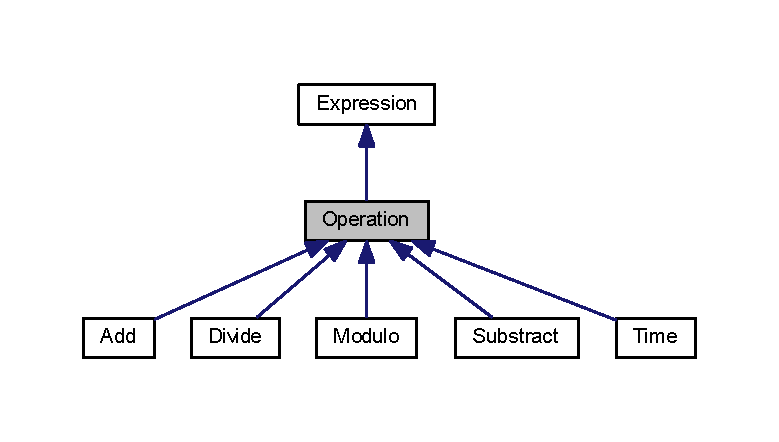
\includegraphics[width=350pt]{class_operation__inherit__graph}
\end{center}
\end{figure}


Collaboration diagram for Operation\-:\nopagebreak
\begin{figure}[H]
\begin{center}
\leavevmode
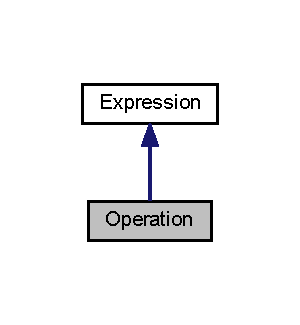
\includegraphics[width=144pt]{class_operation__coll__graph}
\end{center}
\end{figure}
\subsection*{Public Member Functions}
\begin{DoxyCompactItemize}
\item 
\hyperlink{class_operation_a0e3093e2e6de79589f35512d40d3466a}{Operation} (std\-::string body)
\begin{DoxyCompactList}\small\item\em Default constructor. \end{DoxyCompactList}\item 
virtual \hyperlink{class_operation_a14089623bd8a73e73375353c3d8a4b6e}{$\sim$\-Operation} ()
\begin{DoxyCompactList}\small\item\em Default destructor. \end{DoxyCompactList}\item 
\hyperlink{class_expression}{Expression} $\ast$ \hyperlink{class_operation_ace96896e4c65551fa09a2536215b6150}{get\-Left} ()
\begin{DoxyCompactList}\small\item\em Return left part. \end{DoxyCompactList}\item 
\hyperlink{class_expression}{Expression} $\ast$ \hyperlink{class_operation_a5a02d5d55ce671d8dc000a23e030214e}{get\-Right} ()
\begin{DoxyCompactList}\small\item\em Return right part. \end{DoxyCompactList}\item 
void \hyperlink{class_operation_a5ea445954bac8500ce72cc0d3f4e8bb7}{set\-Left} (\hyperlink{class_expression}{Expression} $\ast$left, std\-::list$<$ \hyperlink{class_expression}{Expression} $\ast$ $>$ $\ast$args=N\-U\-L\-L)
\begin{DoxyCompactList}\small\item\em Modify left part. \end{DoxyCompactList}\item 
void \hyperlink{class_operation_aeb66325b8e09adceaebbf7e906e6748c}{set\-Right} (\hyperlink{class_expression}{Expression} $\ast$right, std\-::list$<$ \hyperlink{class_expression}{Expression} $\ast$ $>$ $\ast$args=N\-U\-L\-L)
\begin{DoxyCompactList}\small\item\em Modify right part. \end{DoxyCompactList}\end{DoxyCompactItemize}
\subsection*{Protected Member Functions}
\begin{DoxyCompactItemize}
\item 
void \hyperlink{class_operation_a11cd66e5dbdf38479cff9543a75799ee}{set\-Symbol} (char letter)
\begin{DoxyCompactList}\small\item\em Modify the symbol of this operation. \end{DoxyCompactList}\item 
char \hyperlink{class_operation_ada6e548dc024f08e744b6dc67f76fece}{get\-Symbol} ()
\begin{DoxyCompactList}\small\item\em Return the symbol of the operation. \end{DoxyCompactList}\end{DoxyCompactItemize}
\subsection*{Protected Attributes}
\begin{DoxyCompactItemize}
\item 
\hypertarget{class_operation_a82e0aa90770e887f1471eb04015cc8c7}{std\-::list$<$ \hyperlink{class_expression}{Expression} $\ast$ $>$ $\ast$ {\bfseries m\-\_\-left\-Args}}\label{class_operation_a82e0aa90770e887f1471eb04015cc8c7}

\item 
\hypertarget{class_operation_a7cc352895cd94a1205e0d75288466d7f}{std\-::list$<$ \hyperlink{class_expression}{Expression} $\ast$ $>$ $\ast$ {\bfseries m\-\_\-right\-Args}}\label{class_operation_a7cc352895cd94a1205e0d75288466d7f}

\end{DoxyCompactItemize}


\subsection{Detailed Description}
A\-S\-T \hyperlink{class_operation}{Operation}. 

\begin{DoxyAuthor}{Author}
David Lecoconnier 

Allan Mottier 
\end{DoxyAuthor}
\begin{DoxyDate}{Date}
2013-\/11-\/24 
\end{DoxyDate}


\subsection{Constructor \& Destructor Documentation}
\hypertarget{class_operation_a0e3093e2e6de79589f35512d40d3466a}{\index{Operation@{Operation}!Operation@{Operation}}
\index{Operation@{Operation}!Operation@{Operation}}
\subsubsection[{Operation}]{\setlength{\rightskip}{0pt plus 5cm}Operation\-::\-Operation (
\begin{DoxyParamCaption}
\item[{std\-::string}]{body}
\end{DoxyParamCaption}
)}}\label{class_operation_a0e3093e2e6de79589f35512d40d3466a}


Default constructor. 

Constructor.


\begin{DoxyParams}{Parameters}
{\em body} & text contained \\
\hline
\end{DoxyParams}
\hypertarget{class_operation_a14089623bd8a73e73375353c3d8a4b6e}{\index{Operation@{Operation}!$\sim$\-Operation@{$\sim$\-Operation}}
\index{$\sim$\-Operation@{$\sim$\-Operation}!Operation@{Operation}}
\subsubsection[{$\sim$\-Operation}]{\setlength{\rightskip}{0pt plus 5cm}Operation\-::$\sim$\-Operation (
\begin{DoxyParamCaption}
{}
\end{DoxyParamCaption}
)\hspace{0.3cm}{\ttfamily [virtual]}}}\label{class_operation_a14089623bd8a73e73375353c3d8a4b6e}


Default destructor. 

Destructor. 

\subsection{Member Function Documentation}
\hypertarget{class_operation_ace96896e4c65551fa09a2536215b6150}{\index{Operation@{Operation}!get\-Left@{get\-Left}}
\index{get\-Left@{get\-Left}!Operation@{Operation}}
\subsubsection[{get\-Left}]{\setlength{\rightskip}{0pt plus 5cm}{\bf Expression} $\ast$ Operation\-::get\-Left (
\begin{DoxyParamCaption}
{}
\end{DoxyParamCaption}
)}}\label{class_operation_ace96896e4c65551fa09a2536215b6150}


Return left part. 

\begin{DoxyReturn}{Returns}
left part 
\end{DoxyReturn}
\hypertarget{class_operation_a5a02d5d55ce671d8dc000a23e030214e}{\index{Operation@{Operation}!get\-Right@{get\-Right}}
\index{get\-Right@{get\-Right}!Operation@{Operation}}
\subsubsection[{get\-Right}]{\setlength{\rightskip}{0pt plus 5cm}{\bf Expression} $\ast$ Operation\-::get\-Right (
\begin{DoxyParamCaption}
{}
\end{DoxyParamCaption}
)}}\label{class_operation_a5a02d5d55ce671d8dc000a23e030214e}


Return right part. 

\begin{DoxyReturn}{Returns}
right part 
\end{DoxyReturn}
\hypertarget{class_operation_ada6e548dc024f08e744b6dc67f76fece}{\index{Operation@{Operation}!get\-Symbol@{get\-Symbol}}
\index{get\-Symbol@{get\-Symbol}!Operation@{Operation}}
\subsubsection[{get\-Symbol}]{\setlength{\rightskip}{0pt plus 5cm}char Operation\-::get\-Symbol (
\begin{DoxyParamCaption}
{}
\end{DoxyParamCaption}
)\hspace{0.3cm}{\ttfamily [protected]}}}\label{class_operation_ada6e548dc024f08e744b6dc67f76fece}


Return the symbol of the operation. 

\begin{DoxyReturn}{Returns}
a symbol 
\end{DoxyReturn}
\hypertarget{class_operation_a5ea445954bac8500ce72cc0d3f4e8bb7}{\index{Operation@{Operation}!set\-Left@{set\-Left}}
\index{set\-Left@{set\-Left}!Operation@{Operation}}
\subsubsection[{set\-Left}]{\setlength{\rightskip}{0pt plus 5cm}void Operation\-::set\-Left (
\begin{DoxyParamCaption}
\item[{{\bf Expression} $\ast$}]{left, }
\item[{std\-::list$<$ {\bf Expression} $\ast$ $>$ $\ast$}]{args = {\ttfamily NULL}}
\end{DoxyParamCaption}
)}}\label{class_operation_a5ea445954bac8500ce72cc0d3f4e8bb7}


Modify left part. 


\begin{DoxyParams}{Parameters}
{\em left} & an expression \\
\hline
{\em args} & a list of argument needed by the left eexpression \\
\hline
\end{DoxyParams}
\hypertarget{class_operation_aeb66325b8e09adceaebbf7e906e6748c}{\index{Operation@{Operation}!set\-Right@{set\-Right}}
\index{set\-Right@{set\-Right}!Operation@{Operation}}
\subsubsection[{set\-Right}]{\setlength{\rightskip}{0pt plus 5cm}void Operation\-::set\-Right (
\begin{DoxyParamCaption}
\item[{{\bf Expression} $\ast$}]{right, }
\item[{std\-::list$<$ {\bf Expression} $\ast$ $>$ $\ast$}]{args = {\ttfamily NULL}}
\end{DoxyParamCaption}
)}}\label{class_operation_aeb66325b8e09adceaebbf7e906e6748c}


Modify right part. 


\begin{DoxyParams}{Parameters}
{\em right} & an expression \\
\hline
{\em args} & a list of argument needed by the right eexpression \\
\hline
\end{DoxyParams}
\hypertarget{class_operation_a11cd66e5dbdf38479cff9543a75799ee}{\index{Operation@{Operation}!set\-Symbol@{set\-Symbol}}
\index{set\-Symbol@{set\-Symbol}!Operation@{Operation}}
\subsubsection[{set\-Symbol}]{\setlength{\rightskip}{0pt plus 5cm}void Operation\-::set\-Symbol (
\begin{DoxyParamCaption}
\item[{char}]{letter}
\end{DoxyParamCaption}
)\hspace{0.3cm}{\ttfamily [protected]}}}\label{class_operation_a11cd66e5dbdf38479cff9543a75799ee}


Modify the symbol of this operation. 


\begin{DoxyParams}{Parameters}
{\em letter} & the operation symbol \\
\hline
\end{DoxyParams}


The documentation for this class was generated from the following files\-:\begin{DoxyCompactItemize}
\item 
include/\-Numbers/Operation.\-h\item 
src/\-Numbers/Operation.\-cpp\end{DoxyCompactItemize}

\hypertarget{class_o_r}{\section{O\-R Class Reference}
\label{class_o_r}\index{O\-R@{O\-R}}
}


Or combination.  




Inheritance diagram for O\-R\-:\nopagebreak
\begin{figure}[H]
\begin{center}
\leavevmode
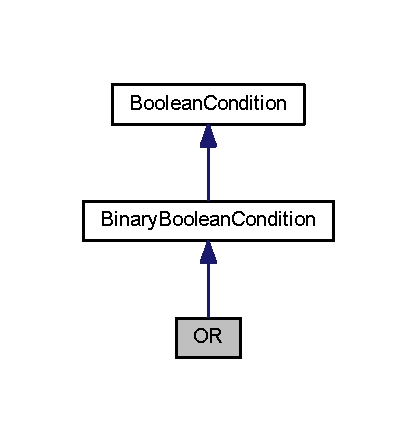
\includegraphics[width=200pt]{class_o_r__inherit__graph}
\end{center}
\end{figure}


Collaboration diagram for O\-R\-:\nopagebreak
\begin{figure}[H]
\begin{center}
\leavevmode
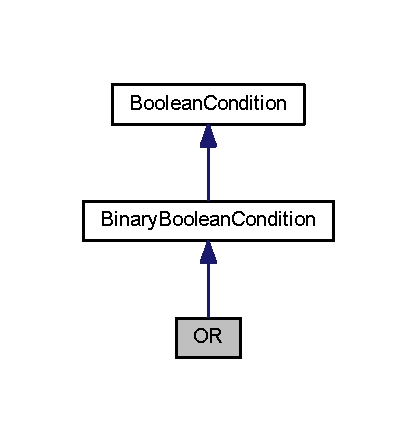
\includegraphics[width=200pt]{class_o_r__coll__graph}
\end{center}
\end{figure}
\subsection*{Public Member Functions}
\begin{DoxyCompactItemize}
\item 
\hyperlink{class_o_r_ab51c726e75cc04a3a56c5b3e339a0a86}{O\-R} (std\-::string body)
\begin{DoxyCompactList}\small\item\em Constructor. \end{DoxyCompactList}\item 
\hypertarget{class_o_r_aed572b0a185eb60b47faba5feb696799}{virtual \hyperlink{class_o_r_aed572b0a185eb60b47faba5feb696799}{$\sim$\-O\-R} ()}\label{class_o_r_aed572b0a185eb60b47faba5feb696799}

\begin{DoxyCompactList}\small\item\em Destructor. \end{DoxyCompactList}\item 
bool \hyperlink{class_o_r_abb0e55c0bd547acd16f09ed88f116078}{eval} ()
\begin{DoxyCompactList}\small\item\em Evaluate the or combination. \end{DoxyCompactList}\end{DoxyCompactItemize}
\subsection*{Additional Inherited Members}


\subsection{Detailed Description}
Or combination. 

\begin{DoxyAuthor}{Author}
David Lecoconnier 

Allan Mottier 
\end{DoxyAuthor}
\begin{DoxyDate}{Date}
2013-\/11-\/24 
\end{DoxyDate}


\subsection{Constructor \& Destructor Documentation}
\hypertarget{class_o_r_ab51c726e75cc04a3a56c5b3e339a0a86}{\index{O\-R@{O\-R}!O\-R@{O\-R}}
\index{O\-R@{O\-R}!OR@{O\-R}}
\subsubsection[{O\-R}]{\setlength{\rightskip}{0pt plus 5cm}O\-R\-::\-O\-R (
\begin{DoxyParamCaption}
\item[{std\-::string}]{body}
\end{DoxyParamCaption}
)}}\label{class_o_r_ab51c726e75cc04a3a56c5b3e339a0a86}


Constructor. 


\begin{DoxyParams}{Parameters}
{\em body} & text contained in I\-F structure \\
\hline
\end{DoxyParams}


\subsection{Member Function Documentation}
\hypertarget{class_o_r_abb0e55c0bd547acd16f09ed88f116078}{\index{O\-R@{O\-R}!eval@{eval}}
\index{eval@{eval}!OR@{O\-R}}
\subsubsection[{eval}]{\setlength{\rightskip}{0pt plus 5cm}bool O\-R\-::eval (
\begin{DoxyParamCaption}
{}
\end{DoxyParamCaption}
)\hspace{0.3cm}{\ttfamily [virtual]}}}\label{class_o_r_abb0e55c0bd547acd16f09ed88f116078}


Evaluate the or combination. 

\begin{DoxyReturn}{Returns}
true if at least one member is true 
\end{DoxyReturn}


Implements \hyperlink{class_boolean_condition}{Boolean\-Condition}.



The documentation for this class was generated from the following files\-:\begin{DoxyCompactItemize}
\item 
include/\-Booleans/O\-R.\-h\item 
src/\-Booleans/O\-R.\-cpp\end{DoxyCompactItemize}

\hypertarget{class_substract}{\section{Substract Class Reference}
\label{class_substract}\index{Substract@{Substract}}
}


\hyperlink{class_substract}{Substract} operation.  




Inheritance diagram for Substract\-:\nopagebreak
\begin{figure}[H]
\begin{center}
\leavevmode
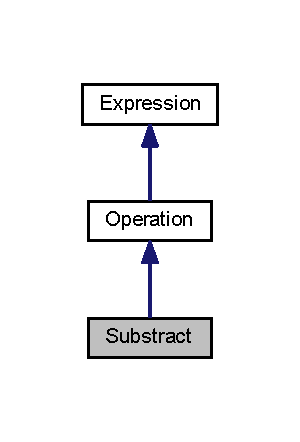
\includegraphics[width=144pt]{class_substract__inherit__graph}
\end{center}
\end{figure}


Collaboration diagram for Substract\-:\nopagebreak
\begin{figure}[H]
\begin{center}
\leavevmode
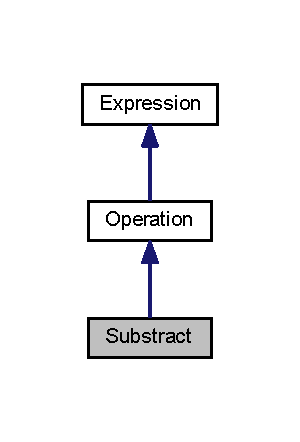
\includegraphics[width=144pt]{class_substract__coll__graph}
\end{center}
\end{figure}
\subsection*{Public Member Functions}
\begin{DoxyCompactItemize}
\item 
\hyperlink{class_substract_a7a2ead7c39ba70ba4db3efaa6e682fcd}{Substract} (std\-::string body)
\begin{DoxyCompactList}\small\item\em Default constructor. \end{DoxyCompactList}\item 
virtual \hyperlink{class_substract_a5f8b67ec608e9f18066c61cf58911c1f}{$\sim$\-Substract} ()
\begin{DoxyCompactList}\small\item\em Default destructor. \end{DoxyCompactList}\item 
virtual \hyperlink{class_abstract_number}{Abstract\-Number} $\ast$ \hyperlink{class_substract_a0293e0b6a390b40496581f039126f4aa}{eval} (std\-::list$<$ \hyperlink{class_expression}{Expression} $\ast$ $>$ $\ast$args)
\begin{DoxyCompactList}\small\item\em Evaluate the \hyperlink{class_substract}{Substract} operation. \end{DoxyCompactList}\end{DoxyCompactItemize}
\subsection*{Additional Inherited Members}


\subsection{Detailed Description}
\hyperlink{class_substract}{Substract} operation. 

\begin{DoxyAuthor}{Author}
David Lecoconnier 

Allan Mottier 
\end{DoxyAuthor}
\begin{DoxyDate}{Date}
2013-\/11-\/24 
\end{DoxyDate}


\subsection{Constructor \& Destructor Documentation}
\hypertarget{class_substract_a7a2ead7c39ba70ba4db3efaa6e682fcd}{\index{Substract@{Substract}!Substract@{Substract}}
\index{Substract@{Substract}!Substract@{Substract}}
\subsubsection[{Substract}]{\setlength{\rightskip}{0pt plus 5cm}Substract\-::\-Substract (
\begin{DoxyParamCaption}
\item[{std\-::string}]{body}
\end{DoxyParamCaption}
)}}\label{class_substract_a7a2ead7c39ba70ba4db3efaa6e682fcd}


Default constructor. 

Constructor.


\begin{DoxyParams}{Parameters}
{\em body} & text contained \\
\hline
\end{DoxyParams}
\hypertarget{class_substract_a5f8b67ec608e9f18066c61cf58911c1f}{\index{Substract@{Substract}!$\sim$\-Substract@{$\sim$\-Substract}}
\index{$\sim$\-Substract@{$\sim$\-Substract}!Substract@{Substract}}
\subsubsection[{$\sim$\-Substract}]{\setlength{\rightskip}{0pt plus 5cm}Substract\-::$\sim$\-Substract (
\begin{DoxyParamCaption}
{}
\end{DoxyParamCaption}
)\hspace{0.3cm}{\ttfamily [virtual]}}}\label{class_substract_a5f8b67ec608e9f18066c61cf58911c1f}


Default destructor. 

Destructor. 

\subsection{Member Function Documentation}
\hypertarget{class_substract_a0293e0b6a390b40496581f039126f4aa}{\index{Substract@{Substract}!eval@{eval}}
\index{eval@{eval}!Substract@{Substract}}
\subsubsection[{eval}]{\setlength{\rightskip}{0pt plus 5cm}{\bf Abstract\-Number} $\ast$ Substract\-::eval (
\begin{DoxyParamCaption}
\item[{std\-::list$<$ {\bf Expression} $\ast$ $>$ $\ast$}]{args}
\end{DoxyParamCaption}
)\hspace{0.3cm}{\ttfamily [virtual]}}}\label{class_substract_a0293e0b6a390b40496581f039126f4aa}


Evaluate the \hyperlink{class_substract}{Substract} operation. 


\begin{DoxyParams}{Parameters}
{\em args} & -\/\-Useless-\/ \\
\hline
\end{DoxyParams}
\begin{DoxyReturn}{Returns}
the result 
\end{DoxyReturn}


Implements \hyperlink{class_expression}{Expression}.



The documentation for this class was generated from the following files\-:\begin{DoxyCompactItemize}
\item 
include/\-Numbers/Substract.\-h\item 
src/\-Numbers/Substract.\-cpp\end{DoxyCompactItemize}

\hypertarget{class_time}{\section{Time Class Reference}
\label{class_time}\index{Time@{Time}}
}


\hyperlink{class_time}{Time} operation.  




Inheritance diagram for Time\-:\nopagebreak
\begin{figure}[H]
\begin{center}
\leavevmode
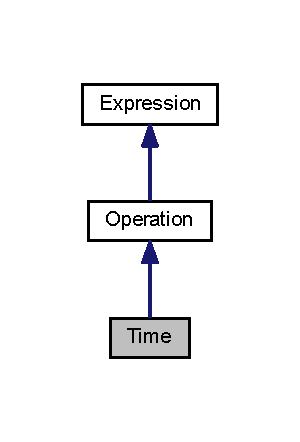
\includegraphics[width=144pt]{class_time__inherit__graph}
\end{center}
\end{figure}


Collaboration diagram for Time\-:\nopagebreak
\begin{figure}[H]
\begin{center}
\leavevmode
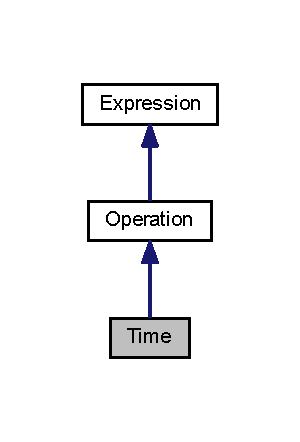
\includegraphics[width=144pt]{class_time__coll__graph}
\end{center}
\end{figure}
\subsection*{Public Member Functions}
\begin{DoxyCompactItemize}
\item 
\hyperlink{class_time_ad2cbdb29f65f86180a83128d6ac3f763}{Time} (std\-::string body)
\begin{DoxyCompactList}\small\item\em Default constructor. \end{DoxyCompactList}\item 
virtual \hyperlink{class_time_a1e92dbe963fa3cdd6bea207680f5f6d1}{$\sim$\-Time} ()
\begin{DoxyCompactList}\small\item\em Default destructor. \end{DoxyCompactList}\item 
virtual \hyperlink{class_abstract_number}{Abstract\-Number} $\ast$ \hyperlink{class_time_a0bbd125f8fa45e351d7f0e2340249071}{eval} (std\-::list$<$ \hyperlink{class_expression}{Expression} $\ast$ $>$ $\ast$args)
\begin{DoxyCompactList}\small\item\em Evaluate the \hyperlink{class_time}{Time} operation. \end{DoxyCompactList}\end{DoxyCompactItemize}
\subsection*{Additional Inherited Members}


\subsection{Detailed Description}
\hyperlink{class_time}{Time} operation. 

\begin{DoxyAuthor}{Author}
David Lecoconnier 

Allan Mottier 
\end{DoxyAuthor}
\begin{DoxyDate}{Date}
2013-\/11-\/24 
\end{DoxyDate}


\subsection{Constructor \& Destructor Documentation}
\hypertarget{class_time_ad2cbdb29f65f86180a83128d6ac3f763}{\index{Time@{Time}!Time@{Time}}
\index{Time@{Time}!Time@{Time}}
\subsubsection[{Time}]{\setlength{\rightskip}{0pt plus 5cm}Time\-::\-Time (
\begin{DoxyParamCaption}
\item[{std\-::string}]{body}
\end{DoxyParamCaption}
)}}\label{class_time_ad2cbdb29f65f86180a83128d6ac3f763}


Default constructor. 

Constructor.


\begin{DoxyParams}{Parameters}
{\em body} & text contained \\
\hline
\end{DoxyParams}
\hypertarget{class_time_a1e92dbe963fa3cdd6bea207680f5f6d1}{\index{Time@{Time}!$\sim$\-Time@{$\sim$\-Time}}
\index{$\sim$\-Time@{$\sim$\-Time}!Time@{Time}}
\subsubsection[{$\sim$\-Time}]{\setlength{\rightskip}{0pt plus 5cm}Time\-::$\sim$\-Time (
\begin{DoxyParamCaption}
{}
\end{DoxyParamCaption}
)\hspace{0.3cm}{\ttfamily [virtual]}}}\label{class_time_a1e92dbe963fa3cdd6bea207680f5f6d1}


Default destructor. 

Destructor. 

\subsection{Member Function Documentation}
\hypertarget{class_time_a0bbd125f8fa45e351d7f0e2340249071}{\index{Time@{Time}!eval@{eval}}
\index{eval@{eval}!Time@{Time}}
\subsubsection[{eval}]{\setlength{\rightskip}{0pt plus 5cm}{\bf Abstract\-Number} $\ast$ Time\-::eval (
\begin{DoxyParamCaption}
\item[{std\-::list$<$ {\bf Expression} $\ast$ $>$ $\ast$}]{args}
\end{DoxyParamCaption}
)\hspace{0.3cm}{\ttfamily [virtual]}}}\label{class_time_a0bbd125f8fa45e351d7f0e2340249071}


Evaluate the \hyperlink{class_time}{Time} operation. 


\begin{DoxyParams}{Parameters}
{\em args} & -\/\-Useless-\/ \\
\hline
\end{DoxyParams}
\begin{DoxyReturn}{Returns}
the result 
\end{DoxyReturn}


Implements \hyperlink{class_expression}{Expression}.



The documentation for this class was generated from the following files\-:\begin{DoxyCompactItemize}
\item 
include/\-Numbers/Time.\-h\item 
src/\-Numbers/Time.\-cpp\end{DoxyCompactItemize}

\hypertarget{class_unary_boolean_condition}{\section{Unary\-Boolean\-Condition Class Reference}
\label{class_unary_boolean_condition}\index{Unary\-Boolean\-Condition@{Unary\-Boolean\-Condition}}
}


Represents an unary boolean condition. It contains one member.  




Inheritance diagram for Unary\-Boolean\-Condition\-:\nopagebreak
\begin{figure}[H]
\begin{center}
\leavevmode
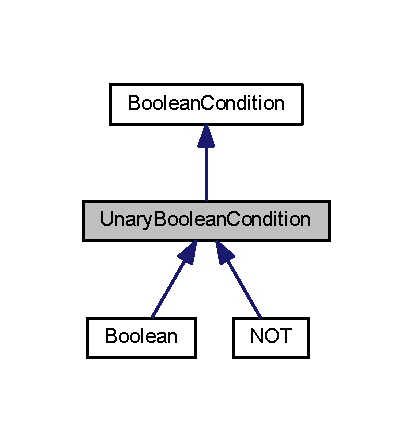
\includegraphics[width=198pt]{class_unary_boolean_condition__inherit__graph}
\end{center}
\end{figure}


Collaboration diagram for Unary\-Boolean\-Condition\-:\nopagebreak
\begin{figure}[H]
\begin{center}
\leavevmode
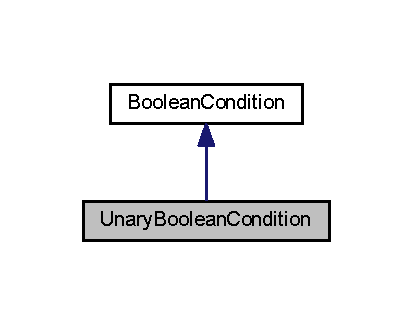
\includegraphics[width=198pt]{class_unary_boolean_condition__coll__graph}
\end{center}
\end{figure}
\subsection*{Public Member Functions}
\begin{DoxyCompactItemize}
\item 
\hyperlink{class_unary_boolean_condition_a824a0171589b68add7c6f31cb05febe1}{Unary\-Boolean\-Condition} (std\-::string body)
\begin{DoxyCompactList}\small\item\em Constructor. \end{DoxyCompactList}\item 
\hypertarget{class_unary_boolean_condition_a1e7896edbf2f52cb4471c53adef7f19e}{virtual \hyperlink{class_unary_boolean_condition_a1e7896edbf2f52cb4471c53adef7f19e}{$\sim$\-Unary\-Boolean\-Condition} ()}\label{class_unary_boolean_condition_a1e7896edbf2f52cb4471c53adef7f19e}

\begin{DoxyCompactList}\small\item\em Destructor. \end{DoxyCompactList}\item 
virtual void \hyperlink{class_unary_boolean_condition_a9927df5d1c8f15fbf1140699c2af7fb7}{set\-Booolean\-Condition} (\hyperlink{class_boolean_condition}{Boolean\-Condition} $\ast$bcond)
\begin{DoxyCompactList}\small\item\em Modify the member. \end{DoxyCompactList}\item 
virtual \hyperlink{class_boolean_condition}{Boolean\-Condition} $\ast$ \hyperlink{class_unary_boolean_condition_a200ba843f7570df93615f37632925db4}{get\-Cond} ()
\begin{DoxyCompactList}\small\item\em Return the member. \end{DoxyCompactList}\end{DoxyCompactItemize}
\subsection*{Additional Inherited Members}


\subsection{Detailed Description}
Represents an unary boolean condition. It contains one member. 

\begin{DoxyAuthor}{Author}
David Lecoconnier 

Allan Mottier 
\end{DoxyAuthor}
\begin{DoxyDate}{Date}
2013-\/11-\/24 
\end{DoxyDate}


\subsection{Constructor \& Destructor Documentation}
\hypertarget{class_unary_boolean_condition_a824a0171589b68add7c6f31cb05febe1}{\index{Unary\-Boolean\-Condition@{Unary\-Boolean\-Condition}!Unary\-Boolean\-Condition@{Unary\-Boolean\-Condition}}
\index{Unary\-Boolean\-Condition@{Unary\-Boolean\-Condition}!UnaryBooleanCondition@{Unary\-Boolean\-Condition}}
\subsubsection[{Unary\-Boolean\-Condition}]{\setlength{\rightskip}{0pt plus 5cm}Unary\-Boolean\-Condition\-::\-Unary\-Boolean\-Condition (
\begin{DoxyParamCaption}
\item[{std\-::string}]{body}
\end{DoxyParamCaption}
)}}\label{class_unary_boolean_condition_a824a0171589b68add7c6f31cb05febe1}


Constructor. 


\begin{DoxyParams}{Parameters}
{\em body} & text contained \\
\hline
\end{DoxyParams}


\subsection{Member Function Documentation}
\hypertarget{class_unary_boolean_condition_a200ba843f7570df93615f37632925db4}{\index{Unary\-Boolean\-Condition@{Unary\-Boolean\-Condition}!get\-Cond@{get\-Cond}}
\index{get\-Cond@{get\-Cond}!UnaryBooleanCondition@{Unary\-Boolean\-Condition}}
\subsubsection[{get\-Cond}]{\setlength{\rightskip}{0pt plus 5cm}{\bf Boolean\-Condition} $\ast$ Unary\-Boolean\-Condition\-::get\-Cond (
\begin{DoxyParamCaption}
{}
\end{DoxyParamCaption}
)\hspace{0.3cm}{\ttfamily [virtual]}}}\label{class_unary_boolean_condition_a200ba843f7570df93615f37632925db4}


Return the member. 

\begin{DoxyReturn}{Returns}
the member 
\end{DoxyReturn}
\hypertarget{class_unary_boolean_condition_a9927df5d1c8f15fbf1140699c2af7fb7}{\index{Unary\-Boolean\-Condition@{Unary\-Boolean\-Condition}!set\-Booolean\-Condition@{set\-Booolean\-Condition}}
\index{set\-Booolean\-Condition@{set\-Booolean\-Condition}!UnaryBooleanCondition@{Unary\-Boolean\-Condition}}
\subsubsection[{set\-Booolean\-Condition}]{\setlength{\rightskip}{0pt plus 5cm}void Unary\-Boolean\-Condition\-::set\-Booolean\-Condition (
\begin{DoxyParamCaption}
\item[{{\bf Boolean\-Condition} $\ast$}]{bcond}
\end{DoxyParamCaption}
)\hspace{0.3cm}{\ttfamily [virtual]}}}\label{class_unary_boolean_condition_a9927df5d1c8f15fbf1140699c2af7fb7}


Modify the member. 


\begin{DoxyParams}{Parameters}
{\em bcond} & a boolean condition \\
\hline
\end{DoxyParams}


The documentation for this class was generated from the following files\-:\begin{DoxyCompactItemize}
\item 
include/\-Booleans/Unary\-Boolean\-Condition.\-h\item 
src/\-Booleans/Unary\-Boolean\-Condition.\-cpp\end{DoxyCompactItemize}

\hypertarget{class_variable}{\section{Variable Class Reference}
\label{class_variable}\index{Variable@{Variable}}
}


\hyperlink{class_variable}{Variable} operation.  




Inheritance diagram for Variable\-:\nopagebreak
\begin{figure}[H]
\begin{center}
\leavevmode
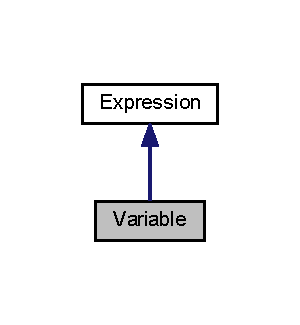
\includegraphics[width=144pt]{class_variable__inherit__graph}
\end{center}
\end{figure}


Collaboration diagram for Variable\-:\nopagebreak
\begin{figure}[H]
\begin{center}
\leavevmode
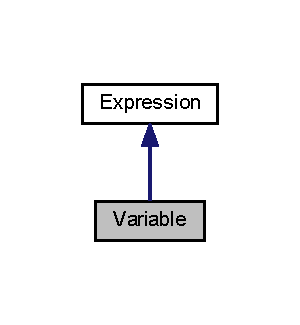
\includegraphics[width=144pt]{class_variable__coll__graph}
\end{center}
\end{figure}
\subsection*{Public Member Functions}
\begin{DoxyCompactItemize}
\item 
\hyperlink{class_variable_a1b8d28ae922899a73e8f2618493bd241}{Variable} (std\-::string body)
\begin{DoxyCompactList}\small\item\em Constructor. \end{DoxyCompactList}\item 
\hypertarget{class_variable_acfc14d0ad77af53025f890b4d3a7745a}{virtual \hyperlink{class_variable_acfc14d0ad77af53025f890b4d3a7745a}{$\sim$\-Variable} ()}\label{class_variable_acfc14d0ad77af53025f890b4d3a7745a}

\begin{DoxyCompactList}\small\item\em Destructor. \end{DoxyCompactList}\item 
std\-::string \hyperlink{class_variable_a63939a8fe4fafe25bb175df35058a6ba}{get\-Name} ()
\begin{DoxyCompactList}\small\item\em Return the name of of the variable. \end{DoxyCompactList}\item 
\hyperlink{class_abstract_number}{Abstract\-Number} $\ast$ \hyperlink{class_variable_a3901741ec3ce0e39923765a8b349c615}{eval} (std\-::list$<$ \hyperlink{class_expression}{Expression} $\ast$ $>$ $\ast$args)
\begin{DoxyCompactList}\small\item\em Evaluate the variable, which means it returns the stored value. \end{DoxyCompactList}\item 
void \hyperlink{class_variable_a3ed8ef37889876fa12fa2fcc0f65512d}{set\-Name} (std\-::string name)
\begin{DoxyCompactList}\small\item\em Modify the name of the variable. \end{DoxyCompactList}\end{DoxyCompactItemize}
\subsection*{Additional Inherited Members}


\subsection{Detailed Description}
\hyperlink{class_variable}{Variable} operation. 

\begin{DoxyAuthor}{Author}
David Lecoconnier 

Allan Mottier 
\end{DoxyAuthor}
\begin{DoxyDate}{Date}
2013-\/11-\/24 
\end{DoxyDate}


\subsection{Constructor \& Destructor Documentation}
\hypertarget{class_variable_a1b8d28ae922899a73e8f2618493bd241}{\index{Variable@{Variable}!Variable@{Variable}}
\index{Variable@{Variable}!Variable@{Variable}}
\subsubsection[{Variable}]{\setlength{\rightskip}{0pt plus 5cm}Variable\-::\-Variable (
\begin{DoxyParamCaption}
\item[{std\-::string}]{body}
\end{DoxyParamCaption}
)}}\label{class_variable_a1b8d28ae922899a73e8f2618493bd241}


Constructor. 


\begin{DoxyParams}{Parameters}
{\em body} & text contained \\
\hline
\end{DoxyParams}


\subsection{Member Function Documentation}
\hypertarget{class_variable_a3901741ec3ce0e39923765a8b349c615}{\index{Variable@{Variable}!eval@{eval}}
\index{eval@{eval}!Variable@{Variable}}
\subsubsection[{eval}]{\setlength{\rightskip}{0pt plus 5cm}{\bf Abstract\-Number} $\ast$ Variable\-::eval (
\begin{DoxyParamCaption}
\item[{std\-::list$<$ {\bf Expression} $\ast$ $>$ $\ast$}]{args}
\end{DoxyParamCaption}
)\hspace{0.3cm}{\ttfamily [virtual]}}}\label{class_variable_a3901741ec3ce0e39923765a8b349c615}


Evaluate the variable, which means it returns the stored value. 


\begin{DoxyParams}{Parameters}
{\em args} & -\/\-Useless-\/ \\
\hline
\end{DoxyParams}
\begin{DoxyReturn}{Returns}
the result 
\end{DoxyReturn}


Implements \hyperlink{class_expression}{Expression}.

\hypertarget{class_variable_a63939a8fe4fafe25bb175df35058a6ba}{\index{Variable@{Variable}!get\-Name@{get\-Name}}
\index{get\-Name@{get\-Name}!Variable@{Variable}}
\subsubsection[{get\-Name}]{\setlength{\rightskip}{0pt plus 5cm}std\-::string Variable\-::get\-Name (
\begin{DoxyParamCaption}
{}
\end{DoxyParamCaption}
)}}\label{class_variable_a63939a8fe4fafe25bb175df35058a6ba}


Return the name of of the variable. 

\begin{DoxyReturn}{Returns}
a name 
\end{DoxyReturn}
\hypertarget{class_variable_a3ed8ef37889876fa12fa2fcc0f65512d}{\index{Variable@{Variable}!set\-Name@{set\-Name}}
\index{set\-Name@{set\-Name}!Variable@{Variable}}
\subsubsection[{set\-Name}]{\setlength{\rightskip}{0pt plus 5cm}void Variable\-::set\-Name (
\begin{DoxyParamCaption}
\item[{std\-::string}]{name}
\end{DoxyParamCaption}
)}}\label{class_variable_a3ed8ef37889876fa12fa2fcc0f65512d}


Modify the name of the variable. 


\begin{DoxyParams}{Parameters}
{\em name} & a name \\
\hline
\end{DoxyParams}


The documentation for this class was generated from the following files\-:\begin{DoxyCompactItemize}
\item 
include/Variable.\-h\item 
src/Variable.\-cpp\end{DoxyCompactItemize}

\addcontentsline{toc}{part}{Index}
\printindex
\end{document}
